\documentclass[11pt,a4]{article}

\parindent=0pt
\parskip=3pt

\setlength{\paperheight}{29.5cm}
\setlength{\paperwidth}{21.2cm}

%\setlength{\voffset}{-2.0cm}
\setlength{\headheight}{0cm}
\setlength{\headsep}{0cm}
\setlength{\textheight}{23.7cm}
\setlength{\textwidth}{16cm}
\setlength{\oddsidemargin}{0cm}
\setlength{\evensidemargin}{0cm}
\setlength{\topmargin}{0cm}
\setlength{\topskip}{0cm}

\catcode`\"=\active \let"=\"
\let\3=\ss

\usepackage[latin9]{inputenc}

\usepackage[sort]{natbib}
\bibpunct{(}{)}{,}{a}{}{,}

\usepackage{amsmath}
\usepackage{amssymb}
\usepackage{amsthm}
\usepackage{IEEEtrantools}
\usepackage{cancel}

%\usepackage[squaren]{SIunits}
\usepackage{graphicx}

%----------------------------------------------------------------------------
%---- Farben und Macros zur Textmarkierung ----------------------------------
%----------------------------------------------------------------------------
\usepackage{color}
\definecolor{light}{gray}{0.50}
\definecolor{heavy}{gray}{0.35}
\definecolor{black}{gray}{0.0}
\definecolor{dgreen}{rgb}{0.0,0.7,0}
\definecolor{dred}{rgb}{0.9959,0,0}
\definecolor{green}{rgb}{0.0,0.99599,0.0}
\definecolor{purple}{rgb}{0.6,0.0,0.4}

\newcommand{\red}[1]{\textcolor{dred}{#1}}
\newcommand{\green}[1]{\textcolor{green}{#1}}
\newcommand{\dgreen}[1]{\textcolor{dgreen}{#1}}
\newcommand{\purple}[1]{\textcolor{purple}{#1}}
\newcommand{\blue}[1]{\textcolor{blue}{#1}}
\newcommand{\black}[1]{\textcolor{black}{#1}}
\newcommand{\grey}[1]{\textcolor{heavy}{#1}}
\newcommand{\lightgrey}[1]{\textcolor{light}{#1}}

\theoremstyle{definition}
\newtheorem{algorithm}{Algorithm}


%----------------------------------------------------------------------------
%---- Kommentare ------------------------------------------------------------
%----------------------------------------------------------------------------

\newcommand{\klein}[1]{\textcolor{blue}{#1}}
\newcounter{kleincommentno}
\setcounter{kleincommentno}{1}
\newcommand{\kleincomment}[1]{{\small\bfseries\textcolor{blue}{ {\small\bfseries${}^{[\arabic{kleincommentno}]}$}}%
\marginpar{\textcolor{blue}{{\small{\bfseries[\arabic{kleincommentno}]}\ \small #1}}\addtocounter{kleincommentno}{1}}}}

\newcommand{\benacchio}[1]{\textcolor{red}{#1}}
\newcounter{benacchiocommentno}
\setcounter{benacchiocommentno}{1}
\newcommand{\benacchiocomment}[1]{{\small\bfseries\textcolor{red}{ {\small\bfseries${}^{[\arabic{benacchiocommentno}]}$}}%
\marginpar{\textcolor{red}{{\small{\bfseries[\arabic{benacchiocommentno}]}\ \small #1}}\addtocounter{benacchiocommentno}{1}}}}

%----------------------------------------------------------------------------
%---- Eigene Macros ---------------------------------------------------------
%----------------------------------------------------------------------------
\newcommand{\hsc}{h_{\rm sc}}
\newcommand{\order}[1]{^{(#1)}}
\let\dss=\displaystyle

\renewcommand{\vector}[1]{\relax\ifmmode\mathchoice
{\mbox{\boldmath$\displaystyle#1$}}
{\mbox{\boldmath$\displaystyle#1$}}
{\mbox{\boldmath$\scriptstyle#1$}}
{\mbox{\boldmath$\scriptscriptstyle#1$}}\else
\hbox{\boldmath$\textstyle#1$}\fi}

\newcommand{\eq}[1]{(\ref{#1})}

\newcommand{\cbar}{\overline{c}}
\newcommand{\thetabar}{\overline{\theta}}
\newcommand{\thetatilde}{\widetilde{\theta}}

\newcommand{\vk}{\vector{k}}
\newcommand{\vu}{\vector{u}}
\newcommand{\vv}{\vector{v}}
\newcommand{\vx}{\vector{x}}

\newcommand{\vV}{\vector{V}}

\newcommand{\ubar}{\overline{u}}
\newcommand{\vbar}{\overline{v}}

\newcommand{\advection}[1]{\mathcal{A}\left[#1\right]}
\newcommand{\advectionNum}[1]{\widetilde{\mathcal{A}}\left[#1\right]}
\newcommand{\rhs}[1]{\mathcal{R}\left[#1\right]}
\newcommand{\source}[1]{S\left(#1\right)}
\newcommand{\Id}{{\rm Id}}

\newcommand{\pprime}{p'}
\newcommand{\halff}{\frac{1}{2}}
\newcommand{\half}{1/2}
\newcommand{\quart}{\frac{1}{4}}
\newcommand{\eightth}{\frac{1}{8}}

\newcommand{\ie}{\emph{i.e.}}

\newcommand{\Nsq}{N^2}
\newcommand{\Nscsq}{(\tau N)^2}

\newcommand{\chibar}{\overline{\chi}}
\newcommand{\chitilde}{{\widetilde \chi}}
\newcommand{\chiprime}{{\chi'}}
\newcommand{\Xtilde}{{\widetilde X}}
\newcommand{\Thetabar}{\overline{\Theta}}
\newcommand{\Thetatilde}{{\widetilde \Theta}}
\newcommand{\pibar}{\overline{\pi}}
\newcommand{\pitilde}{{\widetilde \pi}}
\newcommand{\pihat}{\widehat{\pi}}
\newcommand{\piprime}{\pi'}
\newcommand{\piprimehat}{\widehat{\pi}'}

\newcommand{\Uhat}{\widehat{U}}

\newcommand{\pp}[2]{\frac{\partial #1}{\partial #2}}
\newcommand{\ppn}[3]{\frac{\partial^{#1} #2}{\partial #3^{#1}}}

\newcommand{\bigoh}[1]{\mathcal{O}\left(#1\right)}
\newcommand{\littleoh}[1]{{\scriptstyle\mathcal{O}}\left(#1\right)}

\newcommand{\reals}{\mathbb{R}}

\newcommand{\eps}{\varepsilon}
\newcommand{\rbeta}{\red{\vector{\beta}}}
\newcommand{\balpha}{\blue{\vector{\alpha}}}

\newcommand{\Lopfirst}{{\cal L}^{\rm 1st}}

%\newcommand{\Sol}{\boldsymbol{\mathcal{U}}}
\newcommand{\Sol}{\mathcal{U}}

\newcommand{\rfr}[1]{#1_{\text{ref}}}

\newcommand{\nablatilde}{{\widetilde\nabla}}

\newcommand{\dx}{{\Delta x}}
\newcommand{\dy}{{\Delta y}}
\newcommand{\dz}{{\Delta z}}
\newcommand{\dt}{{\Delta t}}


% ===========================================================================
% ===========================================================================
% ===========================================================================
% ===========================================================================



\title{``Catchy Name''�-- Semi-implicit gravity}
\author{T.~Benacchio, MetOffice, Exeter, UK\\ 
        R.~Klein, Mathematics \& Informatics, Freie Universit\"at Berlin}

\begin{document}

\maketitle

\abstract{
Key points of the paper: 

\begin{itemize}
\item Semi-implicit scheme, only advection explicit
\item Full variables advanced in time
\item Unconditional time step stability w.r.t.\ acoustics, internal waves, Rossby waves
\item Background states \& perturbation variables are only auxiliary
\item Mix of implicit midpoint and implicit trapezoidal rules
\item Borrowing ideas from EULAG/FVM
\benacchio{\item (Mass-, horizontal momentum-,...?) Conservative  \item Second-order \item No off-centering}
\item Further aim: Step towards extending compr/psinc blended model formulation 
      from \citep{BenacchioEtAl2014} to cover hydrostasy, geostrophy, as well
      \citep[see][]{KleinBenacchio2016}.
\end{itemize}
}


% ===========================================================================
% ===========================================================================
% ===========================================================================

\section{Introduction}
\label{sec:Intro}



% ===========================================================================
% ===========================================================================

\subsection{Governing equations}
\label{ssec:GoverningEquations}

The governing equations for adiabatic compressible flow of an inert ideal gas 
with constant specific heat capacities under the influence of gravity and in 
a rotating coordinate system corresponding to a tangent plane approximation
may be written as
%
\begin{IEEEeqnarray}{rCl}\label{eq:CompressibleEuler}
\dss \rho_t + \nabla_\parallel\cdot(\rho \vu) + (\rho w)_z
  & = 
    & \dss 0
      \IEEEyesnumber\IEEEyessubnumber*\label{eq:EulerMass}\\[5pt]
\dss (\rho\vu)_t + \nabla_\parallel\cdot(\rho \vu\circ\vu) + (\rho w \vu)_z 
  & = 
    & \dss - \left( c_p  P \nabla_\parallel \pi + f(y) \vk \times \rho\vu \right)
      \label{eq:EulerHorMom}\\[5pt]
\dss (\rho w)_t + \nabla_\parallel\cdot(\rho \vu w) + (\rho w^2)_z 
  & = 
    & \dss - \left(  c_p P \pi_z + \rho g \right)
      \label{eq:EulerVerMom}\\[5pt]
\dss P_t + \nabla_\parallel\cdot(P\vu) + (Pw)_z
  & = 
    & \dss 0\,.
    \label{eq:EulerPressure}
\end{IEEEeqnarray}
%
Here $\rho$ is the density, $\vu = (u,v)$ and $w$ are the horizontal and vertical 
components of the flow velocity, respectively,  
%
\begin{equation}\label{eq:EOSpiP}
\pi = \left(\frac{p}{\rfr{p}}\right)^{\frac{R}{c_p}}
\qquad\text{and}\qquad
P = \frac{\rfr{p}}{R} \left(\frac{p}{\rfr{p}}\right)^{\frac{c_v}{c_p}} \equiv \rho\Theta
\end{equation}
%
are the Exner pressure and the density weighted potential temperature, respectively, 
with $\rfr{p}$ a suitable reference pressure, $R$ the gas constant and $c_p$ and 
$c_v = c_p - R$ the 
specific heat capacities at constant pressure and constant volume. Furthermore, $g$ is the
(constant) acceleration of gravity, $f(y) = f_0 + \beta y$ the local Coriolis parameter in 
the ``$\beta$-plane'' with suitable constants $f_0$ and $\beta$, $\vk$ the vertical 
unit vector, and $\times$ the cross product. Subscripts as in 
$U_x \equiv \partial_x U := \partial U/ \partial x$ denote partial derivatives with respect 
to the first coordinate of a cartesian $(x,y,z)$ coordinate system or time $t$, and 
$\nabla_\parallel = (\partial_x, \partial_y, 0)$ subsumes the horizontal derivatives.

Given \eq{eq:EulerMass} and \eq{eq:EulerPressure}, the potential temperature
$\Theta = P/\rho$ satisfies the usual advection equation
%
\begin{equation}
\Theta_t + \vu\cdot\nabla_\parallel \Theta + w \Theta_z = 0\,.
\end{equation}

% ===========================================================================
% ===========================================================================

\subsection{Perturbation vs.\ full variables and conservation form}
\label{ssec:PertFullCons}

\klein{Here we should point out difficulties others have had in formulating
a scheme that systematically advances full variables, and in formulating
a scheme in conservation form that is implicit w.r.t.\ buoyancs (e.g.,
Hilary's MWR paper). See ``key points'' in the abstract section.}

% ===========================================================================
% ===========================================================================

\subsection{EULAG: Implicit trapezoidal rule applied along Lagrangian trajectories}
\label{ssec:EULAG}

The semi-implicit time integration procedure implemented in EULAG, 
\citep{PrusaEtAl2008}, and in the more recent finite volume framework for
numerical weather forecasting, FVM, of the European Centre for Medium Range
Weather Forecasting ECMWF, \citep{SmolarkiewiczEtAl2014,KuehnleinEtAl2018}, 
relies on introducing a perturbation potential temperature via
%
\begin{equation}\label{eq:ThetaSplit}
\Theta(t,\vx,z) = \Thetatilde(t,\vx,z) + \Thetabar(z)
\end{equation}
%
and reformulating \eq{eq:CompressibleEuler} as
%
\begin{IEEEeqnarray}{rCrCl}\label{eq:EULAGCompressibleEuler}
\dss \rho_t 
  & + 
    & \dss \nabla_\parallel\cdot(\rho\vu) + (\rho w)_z \hfil
      & = 
        & \dss 0
          \IEEEyesnumber\IEEEyessubnumber*\label{eq:EULAGRhoEqn}\\[5pt]
\dss (\rho\vu)_t 
  & + 
    & \dss \nabla_\parallel\cdot(\rho\vu\circ\vu) + (\rho w\,\vu)_z  \hfil
      & = 
        & \dss - \left( c_p \rho\Theta\nabla_\parallel \pi + f(y) \vk\times\rho\vu\right)
          \label{eq:EULAGHorMomEqn}\\[5pt]
\dss (\rho w)_t 
  & + 
    & \dss \nabla_\parallel\cdot(\rho\vu\, w) + (\rho w\, w)_z \hfil
      & = 
        & \dss - \left( c_p  \rho\Theta \pi_z + \rho g\right)
          \\[5pt]
\dss (\rho\Thetatilde)_t 
  & + 
    & \dss \nabla_\parallel\cdot(\rho\vu\, \Thetatilde) + (\rho w\, \Thetatilde)_z \hfil
      & = 
        & \dss -\left[\nabla_\parallel\cdot(\rho\vu\, \Thetabar) + (\rho w\, \Thetabar)_z\right]\,.
        \label{eq:EULAGThetaTildeEqn}
\end{IEEEeqnarray}
%
In a compact notation, these equations combine the mass balance from \eq{eq:EULAGRhoEqn} with
%
\begin{IEEEeqnarray}{rCl}\label{eq:RhoBasedAdvection}
(\rho\Phi)_t + \mathcal{A}(\Phi; \rho\vv) 
  & = 
    & R(\Phi; \rho)\, ,
\end{IEEEeqnarray}
%
where
%
\begin{equation}\label{eq:EULAGPhiDefinition}
\Phi = (\vu, w, \Thetatilde)^t\, ,
\end{equation}
%
and where $\mathcal{A}(\Phi; \rho\vv)$ denotes the advection terms on the left of
\eq{eq:EULAGHorMomEqn}--\eq{eq:EULAGThetaTildeEqn}, while and $R(\Phi, \rho)$ 
collects all terms on the right. 

Based on this notation, an update of the solution from time $t^n$ to time $t^{n+1}$ according
to their non-oscillatory forward-in-time integration strategy, translated to a simple 
cartesian coordinate setting, then involves first the determination of velocities at the 
half time level via
%
\begin{equation}\label{eq:EULAGFluxExtrapolation}
\vv^{n+\half} = \frac{3}{2} \vv^{n} - \frac{1}{2}  \vv^{n-1}
\end{equation}
%
and the computation of the new time level density
%
\begin{equation}
\rho^{n+1} 
= 
\rho^{n} + \dt\, \nablatilde \cdot (\rho\vv)^{n+\half}
\equiv \mathcal{A}_{\text{\tiny MPDATA}}^{\dt}\left(\rho^n; \vv^{n+1/2}\right)\,,
\end{equation}
%
using their robust, second-order accurate MPDATA%
\footnote{Multidimensional Positive Definite Advection Transport Algorithm}
transport scheme \citep[see, e.g.,][]{SmolarkiewiczMPDATA2006}. Here
$\nablatilde \cdot$ is the standard centered discrete finite volume divergence 
approximation. The mass flux densities, $(\rho\vv)^{n+\half}$, that arise in 
this step are stored for later use in advecting the specific variables $\Phi$ 
defined in \eq{eq:EULAGPhiDefinition}, again with (a variant of) the MPDATA scheme. 
The full update of $\Phi$ then involves the following three-step procedure, 
%
\begin{IEEEeqnarray}{rCl}\label{eq:EULAGTimeIntegrator}
\dss (\rho\Phi)^{*} 
  & = 
    & \dss (\rho\Phi)^{n} + \frac{\dt}{2} R\left(\Phi^n; \rho^n\right)
      \IEEEyesnumber\IEEEyessubnumber*\label{eq:EULAGExplicitEulerStep}\\
\dss (\rho\Phi)^{**} 
  & = 
    & \dss \mathcal{A}_{\text{\tiny MPDATA}}^{\dt}\left(\Phi^*; (\rho\vv)^{n+1/2}\right)
      \label{eq:EULAGAdvectionStep}\\
\dss (\rho\Phi)^{n+1} 
  & = 
    & \dss (\rho\Phi)^{**} + \frac{\dt}{2} R\left(\Phi^{n+1}; \rho^{n+1}\right)\,.
      \label{eq:EULAGImplicitEulerStep}
\end{IEEEeqnarray}
%

We note in passing that the extrapolation scheme for determining the velocities 
$\vv^{n+\half}$ from \eq{eq:EULAGFluxExtrapolation}, which is the default option in EULAG, 
makes the method a three time level�scheme. 
An alternative two time level variant instead carries out an intermediate, at 
least first order accurate, time step of the full equations from $t^{n}$ to $t^{n+1/2}$ and
thus generates $\vv^{n+\half}$ without a need to recur to the $t^{n-1}$ 
level solution. To maintain the large time step stability of the overall semi-implicit
scheme, however, this alternative comes with the cost of an additional elliptic solve for
an intermediate pressure variable per time step. 

Following \citet{SmolarkiewiczMargolin1997}, the scheme in 
\eq{eq:EULAGTimeIntegrator} may be interpreted as the application of the implicit 
trapezoidal rule for time integrating the compatibility condition  
$D\Phi/Dt \equiv (\partial_t + \vv\cdot\nabla) \Phi = R(\Phi; \rho)/\rho$ 
that holds along Lagrangian characteristics of \eq{eq:EULAGCompressibleEuler}.  
Thus, a forward Euler step is followed by a backward Euler step, with the advection 
step interleaved to capture the advancement of the Lagrangian paths. 

An observation that may in part explain the outstanding large time step 
stability features of this scheme is that for given advecting flux $(\rho\vv)^{n+\half}$ 
the advection step is \emph{linear}. As a consequence, even if, for rather large time 
steps, the velocities computed in the forward Euler step \eq{eq:EULAGExplicitEulerStep} 
end up far away from the solutions at time levels $n$ or $n+1$ for large $\dt$, 
these excursions do (i) not affect the advecting fluxes $(\rho\vv)^{n+1/2}$, and they 
can (ii) properly be post-corrected and pulled back to the reasonable range by the 
backward Euler step in \eq{eq:EULAGImplicitEulerStep}. 

% ===========================================================================
% ===========================================================================
% ===========================================================================

\section{Compact description of the time integration scheme}
\label{sec:TimeDiscretizationSummary}

% ===========================================================================
% ===========================================================================

\subsection{Reformulation of the governing equations}
\label{ssec:Reformulation}

% ===========================================================================

\subsubsection{Evolution of the primary variables}
\label{sssec:PrimaryVariables}

The primary unknowns advanced in time by the present scheme are the same as
in \eq{eq:CompressibleEuler}, i.e., $(\rho, \rho\vu, \rho w, P)$. 
Introducing a seamless ``blended'' discretization of the compressible and
pseudo-incompressible \citep{Durran1989} Euler equations and following
\citep{KleinTCFD2009,KleinEtAl2010}, \citet{BenacchioEtAl2014} observed that 
the pseudo-incompressible model is obtained from the compressible equations in 
\eq{eq:CompressibleEuler} by simply dropping the time derivative of 
$P = \rho\Theta$ from \eq{eq:EulerPressure}. To take advantage of this simple 
structural model relationship in constructing a blended scheme that can be
tuned seamlessly from solving the full compressible model equations
to solving the 
pseudo-incompressible model equations, they introduced the inverse of the 
potential temperature,
%
\begin{equation}
\chi = 1/\Theta\,,
\end{equation}
% 
and recast the mass balance \eq{eq:EulerMass} as a transport equation for $\chi$, 
%
\begin{equation}\label{eq:chiI}
\rho_t + \nabla_\parallel\cdot(\rho \vu) + (\rho w)_z = 
(P\chi)_t + \nabla_\parallel\cdot(P\chi \vu) + (P\chi w)_z = 0\,,
\end{equation}
%
in which the field $(P\vv)$ now takes the role of an ``advecting flux''. 
Using this interpretation consistently throughout the equation system we obtain, 
%
\begin{IEEEeqnarray}{rCrCl}\label{eq:EulerP}
\dss \rho_t 
  & + 
    & \dss \nabla_\parallel\cdot(P\vu\, \chi) + (Pw\, \chi)_z \hfil
      & = 
        & \dss 0
          \IEEEyesnumber\IEEEyessubnumber*\label{eq:EulerPMass}\\[5pt]
\dss (\rho\vu)_t 
  & + 
    & \dss \nabla_\parallel\cdot(P\vu\circ\chi\vu) + (Pw\, \chi\vu)_z  \hfil
      & = 
        & \dss - \left( c_p P\nabla_\parallel \pi + f(y) \vk\times\rho\vu\right)
          \label{eq:EulerPHorMom}\\[5pt]
\dss (\rho w)_t 
  & + 
    & \dss \nabla_\parallel\cdot(P \vu\, \chi w) + (Pw\, \chi w)_z \hfil
      & = 
        & \dss - \left( c_p P \pi_z + \rho g\right)
          \label{eq:EulerPVerMom}\\[5pt]
P_t
  &  +
    & \dss \dss \nabla_\parallel\cdot(P\vu)  + (Pw)_z  \hfil
      & = 
        & \dss 0\,.
        \label{eq:EulerPP}
\end{IEEEeqnarray}
%
This formulation is the basis for the discretization proposed below, which
is to lay the foundationd for extending the seamless compressibility-related
model blending of \citet{BenacchioEtAl2014} also to hydrostasy and geostrophy. 

% ===========================================================================

\subsubsection{Auxilary perturbation variables and evolution equations}
\label{sssec:AuxPerturbationVariables}

A crucial ingredient of any scheme that is implicit with respect to the 
effects of compressibility, buoyancy, and Earth rotation, is separate 
access to the large-scale mean background stratifications of pressure and 
potential temperature, or its inverse, and to their local perturbations. 
Thus, in analogy with \eq{eq:ThetaSplit} we split the Exner pressure $\pi$ 
and inverse potential temperature $\chi$ into
%
\begin{equation}\label{eq:PerturbationVariables}
\pi(t,\vx,z) = \piprime(t,\vx,z) + \pibar(z)
\qquad\text{and}\qquad
\chi(t,\vx,z) = \chiprime(t,\vx,z) + \chibar(z)\, ,
\end{equation}
% 
where the background variables satisfy the hydrostatic relation
%
\begin{equation}\label{eq:BackgroundHydrostatics}
\frac{d\pibar}{dz} = - \frac{g}{c_p} \chibar
\qquad\text{with}\qquad
\pibar(0) = 1\, .
\end{equation}
%

Since $P$ can be expressed as a function of $\pi$ alone according to
\eq{eq:EOSpiP} and as $\pibar$ is time independent across a time step, 
the perturbation Exner pressure satisfies
%
\begin{equation}\label{eq:EulerPiPrime}
\left(\frac{\partial P}{\partial \pi}\right) \piprime_t
= 
- \nabla\cdot (P(\pi)\vv)\,,
\end{equation}
%
which is a direct consequence of \eq{eq:EulerPP}.
In turn, the perturbation form of the mass balance serves as the evolution equation
for $\chiprime$, i.e.,
%
\begin{IEEEeqnarray}{rCrCl}\label{eq:EulerPChiPrime}
\dss (P\chiprime)_t 
  & + 
    & \dss \nabla_\parallel\cdot(P\vu\, \chiprime) + (Pw\, \chiprime)_z \hfil
      & = 
        & \dss -\left[\nabla_\parallel\cdot(P\vu\, \chibar) + (Pw\, \chibar)_z\right]\,.
        \label{eq:ChiPrimeEqn}
\end{IEEEeqnarray}
%

Auxiliary discretizations of \eq{eq:EulerPiPrime} and 
\eq{eq:EulerPChiPrime} will be used in constructing a numerical scheme
for the full variable form of the governing equations in \eq{eq:EulerP}
that is stable for time steps limited only by the advection Courant 
number. After completion of a time step, the perturbation variables
are synchronized with the full variables based on the definitions
in \eq{eq:PerturbationVariables} and \eq{eq:BackgroundHydrostatics}.
\benacchio{We should perhaps better clarify how this makes the scheme
different from all the other models that work with perturbations only,
e.g. ENDGame works with the old time-step profiles as reference. In our case
the decompositions \eq{eq:PerturbationVariables} and \eq{eq:BackgroundHydrostatics} are only
instrumental to constructing the elliptic problems in the correction steps.
I shall go into the bells and whistles of other schemes to understand how
they carry forward perturbations more than we do.} \klein{That will be 
very much appreciated! We need to be careful and don't want to claim too
much in the end.}

In the sequel, borrowing notation from \citet{SmolarkiewiczEtAl2014},
see section~\ref{ssec:EULAG}, we introduce
%
\begin{equation}\label{eq:PsiDefinition}
\Psi = (\chi, \chi\vu, \chi w, \chiprime)
\end{equation}
%
and subsume the primary equations in \eq{eq:EulerP} and the auxiliary 
equation for $\chiprime$ in \eq{eq:ChiPrimeEqn} as 
%
\begin{IEEEeqnarray}{rCl}\label{eq:PBasedAdvection}
(P\Psi)_t + \mathcal{A}(\Psi; P\vv) 
  & = 
    & Q(\Psi; P)
      \IEEEyesnumber\IEEEyessubnumber*\label{eq:EulerPCompactPsi}\\
P_t + \nabla\cdot(P\vv)
  & =
    & 0\,.
    \label{eq:EulerPCompactP}
\end{IEEEeqnarray}
%
Note that the $\pi'$ evolution equation in \eq{eq:EulerPiPrime} is 
equivalent to \eq{eq:EulerPCompactP} and need not be listed separately.

% ===========================================================================
% ===========================================================================

\subsection{Summary of the semi-implicit time discretization}
\label{ssec:TimeDiscretizationOverview}


\klein{Tommaso, please check critically whether you find the birds-eye
view of the scheme presented in this section useful at all. It might 
appear a bit odd upon first reading, but be helpful as a reference on
the overall structure when reading the more detailed material further down. 
But it might also simply be confusing. I am not sure.}

% ===========================================================================

\subsubsection{(Semi-)implicit midpoint pressure update and advective fluxes}
\label{sssec:AdvectiveFluxes}

The first step in our scheme is the determination of advective fluxes 
at the half-time level, $(P\vv)^{n+\half}$, which immediately yield the
update of the internal energy variable, $P$, through
%
\begin{equation}\label{eq:PUpdate}
P^{n+1} 
= 
P^{n} - \dt \,\nablatilde\cdot(P\vv)^{n+\half}\,.
\end{equation}
%
where $\nablatilde \cdot$ is again the discrete approximation of the divergence.
\klein{Note that this update corresponds to a time discretization of this equation
using the \emph{implicit midpoint rule}. We recall here for future reference that
an implementation of the implicit midpoint rule can be achieved by first applying
a half time step based on the implicit Euler scheme followed by another half time
step based on the explicit Euler method \citep{HairerEtAl2006}.}

To maintain second order accuracy of the overall scheme, a first order accurate 
time integration from the last completed time step at $t^n$ is sufficient for 
generating these half time level fluxes. \klein{[OK, here is a brief explanation:]} 
This becomes transparent through a truncation error analysis for any equation of 
the form $\dot y = R(y,t)$. First we observe that
%
\begin{equation}\label{eq:FirstOrderHTLUpdateI}
\frac{y(t^{n+1})-y(t^n)}{\dt} = \dot y\left(t^{n+\half}\right) + \bigoh{\dt^2}
\end{equation}
%
by straightforward Taylor expansion. Then, for any first-order approximation, 
say $R^{n+\half}$, to the right hand side at the half time level we have  
%
\begin{equation}\label{eq:FirstOrderHTLUpdateII}
\dot y\left(t^{n+\half}\right) 
= R\left(y\left(t^{n+\half}\right)\right) 
= R\left(y(t^n)\right) + \delta R^n + \bigoh{\dt^2} 
=: R^{n+\half} + \bigoh{\dt^2}\,.
\end{equation}
%
Re-inserting into \eq{eq:FirstOrderHTLUpdateI} we find
%
\begin{equation}
\frac{y(t^{n+1})-y(t^n)}{\dt} = R^{n+\half} + \bigoh{\dt^2}\, ,
\end{equation}
%
which indicates that second order accuracy can be achieved when the right hand
side is locally approximated at the half time level only by a first order update
from the old time level.  

To achieve
stability for large time steps, limited only by the advection Courant number,
we invoke standard splitting into advective and non-advective terms in 
\eq{eq:EulerP}, \eq{eq:EulerPChiPrime}, with explicit advection and 
linearly implicit treatment of the right hand sides. 
Thus we first advance the scalars from \eq{eq:PsiDefinition} by half an advection 
time step utilizing advective fluxes computed at the old time level, 
%
\begin{IEEEeqnarray}{rCl}\label{eq:HalfTimePredictorAdvection}
\dss (P\Psi)^{\#} 
  & = 
    & \dss \mathcal{A}_{1\text{st}}^{\frac{\dt}{2}}\left(\Psi^{n}; (P\vv)^{n}\right)
      \IEEEyesnumber\IEEEyessubnumber*\\
\dss P^{\#} 
  & = 
    & \dss P^{n} - \frac{\dt}{2} \nablatilde\cdot(P\vv)^{n}\,.
\end{IEEEeqnarray}
%
Here $\mathcal{A}_{1\text{st}}^{\dt}$ denotes an at least first order
accurate version of our advection scheme (see section~\ref{ssec:Advection}).  
Then, the half time level fluxes $(P\vv)^{n+\half}$ are obtained as a result
of an implicit Euler discretization of the second split system that involves
only the right hand sides of \eq{eq:EulerP} (see 
section~\ref{ssec:SemiImplicitForcing} for details), 
%
\begin{IEEEeqnarray}{rCl}\label{eq:HalfTimePredictorFluxCorrection}
\dss (P\Psi)^{n+\half} 
  & = 
    & \dss (P\Psi)^{\#} + \frac{\dt}{2} Q\left(\Psi^{n+1/2}; P^{n+\half}\right)\,,
      \IEEEyesnumber\IEEEyessubnumber*\label{eq:HalfTimePredictorRHS}\\
\dss P^{n+\half} 
  & = 
    & \dss P^{n} - \frac{\dt}{2} \nabla\cdot(P\vv)^{n+\half}\,.
      \label{eq:HalfTimePredictorDivControl}
\end{IEEEeqnarray}
%
\klein{We note that \eq{eq:HalfTimePredictorDivControl} corresponds to the
implicit Euler update to the half time level, \emph{i.e.}, to the first step of 
our implementation of the implicit midpoint rule for $P$.} 
Furthermore, in this step the 
relation between $P$, which is being updated by the flux divergence, and $\pi$, 
whose gradient is part of the momentum forcing terms, is approximated through a 
linearization of the equations of state \eq{eq:EOSpiP}, i.e.,  
%     
\begin{IEEEeqnarray}{rCl}\label{eq:HalfTimePredictorPLinearization}
\dss P^{n+\half} 
  & = 
    & \dss P^{n} 
      + \left(\frac{\partial P}{\partial \pi}\right)^{\#} 
        \left(\pi^{n+\half} - \pi^{n}\right)\,.
\end{IEEEeqnarray}
%
With this linearization, this implicit Euler step involves a single linear elliptic 
solve for $\pi^{n+\half}$ as will become clear below. Optionally, an outer iteration 
of the linearly implicit step can be invoked to guarantee consistency with the 
equation of state for $P(\pi)$ up to machine accuracy. 

\klein{These preliminary calculations serve to provide the fluxes $(P\vv)^{n+\half}$ 
needed subsequently both for the concluding explicit Euler update of $P$ to the full
time level $t^{n+1}$ and for the advection of the vector of specific variables $\Psi$ 
from \eq{eq:PsiDefinition} as part of the overall time stepping algorithm, 
see \eq{eq:AdvectionStep} below.}

\klein{We note in passing that our treatment of the $P$ variable is quite similar to how 
density updates are handled and mass fluxes are utilized for advection in the 
EULAG/FVM algorithm summarized in section~\ref{ssec:EULAG}.}

% ===========================================================================

\subsubsection{Implicit trapezoidal rule along explicit Lagrangian 
paths for advected scalars}
\label{sssec:FullTimeStep}

Given the advective fluxes, $(P\vv)^{n+\half}$, the full second order 
semi-implicit time step for the evolution equation \eq{eq:RhoBasedAdvection}
of the advected scalars, $\Psi$, reads
%
\begin{IEEEeqnarray}{rCl}\label{eq:TimeIntegrator}
\dss (P\Psi)^{*} 
  & = 
    & \dss (P\Psi)^{n} + \frac{\dt}{2} Q\left(\Psi^n; P^n\right)
      \IEEEyesnumber\IEEEyessubnumber*\label{eq:ExplicitEulerStep}\\
\dss (P\Psi)^{**} 
  & = 
    & \dss \mathcal{A}_{2\text{\tiny nd}}^{\dt}\left(\Psi^*; (P\vv)^{n+1/2}\right)
      \label{eq:AdvectionStep}\\
\dss (P\Psi)^{n+1} 
  & = 
    & \dss (P\Psi)^{**} + \frac{\dt}{2} Q\left(\Psi^{n+1}; P^{n+1}\right)\,.
      \label{eq:ImplicitEulerStep}
\end{IEEEeqnarray}
%
For future reference we notice that the two equations without source term
for $\rho$ and $P$ are not involved in \eq{eq:ExplicitEulerStep} and
\eq{eq:ImplicitEulerStep}. The updates to $\rho^{n+1}$ and $P^{n+1}$ are
entirely determined by the advection step in \eq{eq:AdvectionStep} and
by the implicit midpoint discretization of the $P$-component in \eq{eq:PUpdate}. 
\klein{In fact, the $P$-component of \eq{eq:AdvectionStep} corresponds to 
completing the implicit midpoint discretization for the $P$-equation.}

\benacchio{From this it seems that \eq{eq:PUpdate} happens after \eq{eq:AdvectionStep},
does it not? Or is it meant \eq{eq:AdvectionStep} for $\rho$(i.e. $P\chi$) and \eq{eq:PUpdate}
for $P$?} \klein{Indeed, you are right. This is what happens. It is the usual 
procedure for the implicit midpoint rule. You first compute the right hand side
at the half time level advancing all variables by the implicit Euler discretization. 
Then you extrapolate the obtained update all the way to the full time level. 
\eq{eq:PUpdate}  -- or better \eq{eq:HalfTimePredictorDivControl} -- corresponds to 
the first Euler backward half time step, while \eq{eq:AdvectionStep} for $P$ 
corresponds to the extrapolation to the full time level.
I have tried to make this more transparent in the above with a few additional sentences.
Please check.}

Therefore, the unknowns that effectively get updated in the explicit and 
implicit Euler steps \eq{eq:ExplicitEulerStep} and \eq{eq:ImplicitEulerStep}, respectively, 
are $(\vu, w, \chiprime)$ only. Nevertheless, to obtain 
an appropriate approximation of the Exner pressure gradient needed in the 
momentum equation, an auxiliary implicit Euler discretization of the energy 
equation in perturbation form for $\piprime$ 

(\benacchio{is this what was the second
projection? \klein{Yes.} ... or both the first and the second? \klein{No.}
It is not completely clear what the
connection is between the new framework and the predictor corrector framework of
Klein(2009) and Benacchio et al. (2014). If the predictor-corrector can be cast into
the explicit-then-implicit framework then perhaps the translation could be detailed,
and I think this is a potential element of novelty as well.} \klein{The first projection
from our earlier scheme corresponds directly with the procedure detailed in 
section~\ref{sssec:AdvectiveFluxes}, the second projection is what happens here.
I agree that we should point out the connections to and differences from our 
earlier approach!}) 

from \eq{eq:EulerPiPrime} is 
utilized in formulating \eq{eq:ImplicitEulerStep}. See 
section~\ref{ssec:SemiImplicitForcing} for details. 

After completion of the steps in \eq{eq:TimeIntegrator}, the
auxiliary variables $(\chiprime, \pi')$ are re-computed from the primary
unknowns $(\rho, \rho\vu, \rho w, P)$ at the new time level.  \klein{[That
actually turns out to fail in some tests. We'll have to discuss this. I get
the best results if I drop the synchronization of cell-centered and nodal
pressures entirely and just update these fields redundantly. Miraculously, 
the stay very close in all tests that I ran. If we could explain this, that
would be great!}
This ensures
consistency of all variables with respect to the equation of state and
ensures that $(\chiprime, \pi')$ are approximated with the same, i.e., 
second, order of accuracy as the primary variables across multiple time 
steps.

Clearly, from the perspective of their bird's-eye views in 
\eq{eq:TimeIntegrator} and \eq{eq:EULAGTimeIntegrator}, the scheme and the 
EULAG/FVM forward-in-time discretization from 
\citep{PrusaEtAl2008,SmolarkiewiczEtAl2014} look like almost identical twins.
This is not a coincidence as the latter served as a reference for the present
developments owing to its impressive stability features and accuracy for 
realistic applications, competitive with even a pseudo-spectral scheme
as demonstrated recently by \citet{KuehnleinEtAl2018}. There are differences,
however, and we discuss these in the conclusions section~\ref{sec:Conclusions} 
below.

% ===========================================================================
% ===========================================================================
% ===========================================================================

\section{Discretization details}
\label{sec:DiscretizationDetails}

% ===========================================================================
% ===========================================================================

\subsection{Cartesian grid arrangement}
\label{ssec:GridArrangement}


\begin{figure}
\centering
 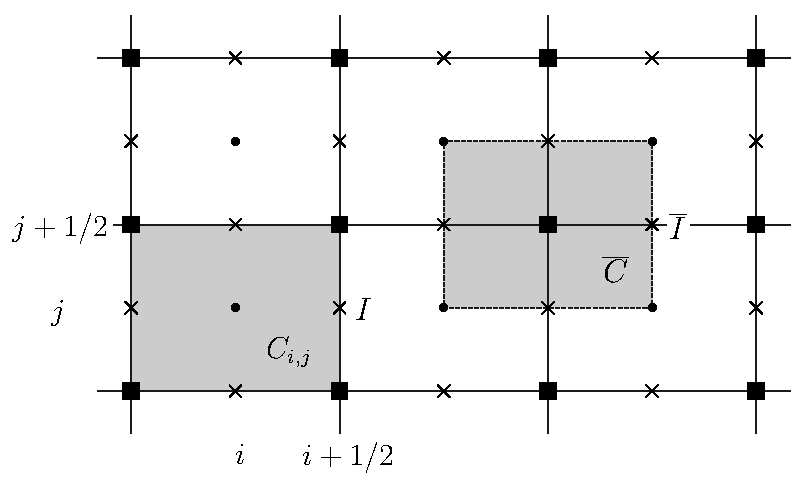
\includegraphics{Graphics/Grid}
\caption{Cartesian grid arrangement for two space dimensions. 
$C_{i,j}$: primary finite volumes, 
$\ \bullet\ $: primary cell centers, $I$: primary cell interfaces,
$\times$: centers of both primary and dual cell interfaces, 
$\overline{C}$: dual cells for nodal pressure computation, $\ \rule[1pt]{4pt}{4pt}\ $:
dual cell centers, $\overline{I}$: dual cell interfaces.
\label{fig:GridArrangement}}
\end{figure}

The space discretization of the present scheme is fully cell centered 
on control volumes $C_{i,j,k}$ formed by a cartesian mesh with constant 
grid increments $\dx, \dy, \dz$, and grid indices $i = 0, ..., I-1$,  
$j = 0, ..., J-1$, $k = 0, ..., K-1$ (see Fig.~\ref{fig:GridArrangement}
for a sketch of a two dimensional $x$-$y$ slice). The primary variables 
of the discrete approximate solution consists of grid cell 
averages 
%
\begin{equation}
\Sol_{i,j,k}^n \approx 
\frac{1}{\dx \dy \dz}\int\limits_{C_{i,j,k}} \Sol(\vx,t^n)\, d^3\vx
\qquad\text{of}\qquad 
\Sol = \left(
\begin{array}{c}
\rho \\ \rho\vu \\ \rho w \\ P \\ P\chiprime
\end{array}
\right)\,.
\end{equation}
%
The scheme is second order accurate, so that -- within the approximation
order -- we can interchangeably interpret $\Sol_{i,j,k}^n$ as the cell average, 
as above, or as a point value of $\Sol$ at the center of mass of the grid 
cell.  

Advection of the specific variables $\Psi$ is mediated by fluxes defined 
on cell faces, i.e.,
%
\begin{equation}\label{eq:DiscreteAdvectiveFluxes}
(Pu \Psi)^{n+\half}_{i+\half,j,k}\,,
\qquad
(Pv \Psi)^{n+\half}_{i,j+\half,k}\,, 
\qquad
(Pw \Psi)^{n+\half}_{i,j,k+\half}\,,
\end{equation}
%
determined by some robust second order advection scheme. See 
section~\ref{sssec:AdvectiveFluxes} for the present implentation using
a ``monotone upwind scheme for conservation laws'' (MUSCL) 
following \citep[see, e.g.,][]{vanLeer2006}. 
The fluxes in \eq{eq:DiscreteAdvectiveFluxes} are staggered-grid 
components of the advective flux field $(P\vv)^{n+\half}$ referred
to in section~\ref{ssec:TimeDiscretizationOverview} above. See
Fig.~\ref{fig:GridArrangement} for their arrangement on the computational 
grid.

Two different incarnations of the Exner pressure gradient are needed in 
the implicit Euler steps summarized in \eq{eq:HalfTimePredictorFluxCorrection} 
and \eq{eq:ImplicitEulerStep}. The former determines the cell interface
based fluxes from \eq{eq:DiscreteAdvectiveFluxes} and naturally works with 
cell- and timestep-centered values of the Exner pressure ($\pi_{i,j,k}^n$). 
The latter corrects the cell-centered momenta and requires integrals of the Exner 
pressure over grid cell faces to form a finite-volume discretization of 
the gradient, and this is computed from node-centered values by the 
trapezoidal rule quadrature. Thus we compute both
%
\begin{equation}\label{eq:ExnerPressures}
\pi_{i,j,k}^{n+\half} 
\qquad\text{and}\qquad
\pi_{i+\half,j+\half,k+\half}^{n+1} 
\end{equation}
%
in the course of a time step $t^{n} \to t^{n+1}$ by solving implicit 
pressure equations. 

% ===========================================================================
% ===========================================================================

\subsection{Synchronization of auxiliary variables}
\label{ssec:Synchronization}

The fluid dynamical pressure $p$ plays multiple roles in the compressible 
Euler equations as formulated in \eq{eq:CompressibleEuler}. The cell-centered 
volume average of $P = (\rfr{p}/R) (p/\rfr{p})^{c_v/c_p}$ is representative 
of the internal energy budget of the flow, whereas the gradient of the Exner 
pressure $\pi = (p/\rfr{p})^{R/c_p}$ arises in the coupling of the momentum 
field to the pressure. As a consequence, the implicit Euler steps control both 
the advective fluxes $(P\vv)^{n+\half}$ at cell faces in 
\eq{eq:HalfTimePredictorFluxCorrection} and the momenta $(\rho \vv)$ at the 
cell centers in \eq{eq:TimeIntegrator}, thereby employing both cell-centered
and node-centered approximations of the Exner pressure, see \eq{eq:ExnerPressures} 
and sections~\ref{sssec:DivControlledAdvectiveFluxes} and 
\ref{sssec:TrapezoidalRule} below. This is in agreement with our previous
developments in \cite{KleinTCFD2009,BenacchioEtAl2014}, and with the 
established combination of ``MAC'' and cell-centered projections for 
zero Mach number flow solvers in \citep[e.g.,][]{BellEtAl1989,AlmgrenEtAl2006}.


These auxiliary fields are synchronized upon completion of the $n$th time
step with the primary cell centered variable $P^n_{i,j}$ through
%
\begin{IEEEeqnarray}{rCl}
\pi^{n}_{i,j,k} 
  & =
    & \left(\frac{RP_{i,j,k}^n}{\rfr{p}}\right)^{\frac{R}{c_v}}
      \IEEEyesnumber\IEEEyessubnumber*\\[10pt]
\pi^{n}_{i+\half,j+\half,k+\half}
  & =
    & \frac{1}{8}
      \sum_{\lambda,\mu,\nu = 0}^1 \pi^{n}_{i+\lambda,j+\mu,k+\nu} \,. 
%      \left(\pi^{n}_{i,j} + \pi^{n}_{i+1,j} + \pi^{n}_{i,j+1} + \pi^{n}_{i+1,j+1} 
%      \right)\,.
      \label{eq:CenterToNodeInterpolation}
\end{IEEEeqnarray}
%
\klein{[As stated earlier, the latter synchronization step is detrimental 
in some tests. Everything works smoothly if I just evolve the nodal pressures
independently of the cell-centered variables. Synchronization of the cell-centered
variables is OK, though. The reason, I surmise, is that the detrimental bit
in \eq{eq:CenterToNodeInterpolation} is the interpolation, which destroys information.]}

\purple{The formula in \eq{eq:CenterToNodeInterpolation} is also used to generate 
half time level nodal pressures from the cell-centered solution 
$\pi^{n+\half}_{i,j,k}$ arising in the advective flux 
calculation scheme in \eq{eq:HalfTimePredictorFluxCorrection}, 
\eq{eq:HalfTimePredictorPLinearization}.} \klein{[That, too, is no longer needed
in the most recent -- and so far best -- version of the scheme.]}

Similarly, the split of the full inverse of the potential temperature 
$\chi = \chiprime + \chibar$ according to \eq{eq:PerturbationVariables} and the subsequent 
separate updates of  $\chi$ and $\chiprime$ governed by discrete versions
of the full and perturbed mass balances in \eq{eq:chiI} and 
\eq{eq:EulerPChiPrime}, respectively, require re-synchronization. Thus, 
after completion of a time step we let
%
\begin{equation}
\chiprime_{i,j,k}^{n} = \chi_{i,j,k}^{n} - \chibar_{k}^{n}\,,
\end{equation}   
%
where we have assumed gravity to be aligned with the $z$-coordinate
direction so that the discrete version of $\chibar(z)$ depends on the 
associated index $k$ only. Also, in 
all subsequent simulations we set $\chibar_k^{n} \equiv \chibar_k^{0}$. 
An alternative option better suited for large scale, long time simulations 
is to invoke a horizontal, possibly local, averaging procedure to extract 
$\chibar$ from $\chi$ at least every few time steps. \benacchio{Unified Model
uses the state at the previous time step, we could perhaps try that as well?} 
\klein{I did, and I found it to be a bad idea: Suppose we wish to simulate
a breaking internal wave that shows local overturning of the potential 
temperature surfaces. This will routinely happen in a high-resolution simulation 
at somewhat higher altitudes. If such a state were used as a reference for 
linearization, $N^2$ would be zero locally, and I think that ellipticity of
the linearized equation for $\pi'$ would be lost.} We leave testing 
this option to future work.	 

% ===========================================================================
% ===========================================================================

\subsection{Advection}
\label{ssec:Advection}

Any robust numerical scheme capable of performing advection of a scalar in
compressible flows is a good candidate for the generic discrete
advection operators $\mathcal{A}_{\text{1st}}^{\dt}$ and 
$\mathcal{A}_{\text{2nd}}^{\dt}$ introduced above. EULAG uses 
variants of the ``multi-dimensional positive definite advection transport 
algorithm'' (MPDATA) \citep{PrusaEtAl2008}. The present implementation involves
a directionally split ``monotone upwind scheme for conservation laws'' (MUSCL)
\citep[see, e.g.,][]{vanLeer2006}: 

Suppose the half time predictor step from \eq{eq:HalfTimePredictorFluxCorrection}, 
the details of which will be described shortly \benacchio{(could we not put the details
- presumably \eq{eq:firstorder_Adv} - here instead and spare the reader a back-reference?)}
\klein{[No, I don't think this helps. It is not just \eq{eq:firstorder_Adv}. We need
the full result $(P\vv)^{n+\half}$ from section~\ref{sssec:AdvectiveFluxes}.]}, 
has been completed. Then, 
the components of the advecting fluxes $(P\vv)^{n+\half}$ at grid cell faces 
have become available as part of this calculation. Given these fluxes, the advection 
step in \eq{eq:AdvectionStep} is discretized via Strang splitting, so that
%
\begin{equation}\label{eq:AdvectionStrangSplitting}
\Sol_{i,j}^{**} 
=
\mathcal{A}_{2\text{nd}}^{\dt} \Sol_{i,j,k}^{*} 
\equiv
\mathcal{A}^{\frac{\dt}{2}}_x 
\mathcal{A}^{\frac{\dt}{2}}_y 
\mathcal{A}^{\frac{\dt}{2}}_z 
\mathcal{A}^{\frac{\dt}{2}}_z 
\mathcal{A}^{\frac{\dt}{2}}_y 
\mathcal{A}^{\frac{\dt}{2}}_x\, \Sol_{i,j}^{*} \,,
\end{equation}
%
where, dropping the indices of the transverse directions 
for transparency of notation, we have, e.g., 
%
\begin{equation}
\mathcal{A}^{\frac{\dt}{2}}_x\, \Sol_{i} 
= \Sol_{i}
- \frac{\dt}{2\dx} 
  \left((Pu)^{n+\half}_{i+\half}\, \Psi_{i+\half} 
      - (Pu)^{n+\half}_{i-\half}\, \Psi_{i-\half} \right)
\end{equation}
%
with 
%
\begin{IEEEeqnarray}{rCl}\label{eq:AdvSpecifics}
\Psi_{i+\half} 
  & = 
    & \sigma \Psi^{-}_{i+\half} + (1-\sigma)\Psi^{+}_{i+\half}\,,
      \IEEEyesnumber\IEEEyessubnumber*\\[8pt]
\sigma 
  & = 
    & \text{sign}\left((Pu)^{n+\half}_{i+\half}\right)\,,
      \\[8pt]
\Psi^{-}_{i+\half} 
  & = 
    & \Psi_{i} + \frac{\dx}{2} \left(1 - C^{n+\half}_{i+\half} \right)  s_{i}\,,
      \\[8pt]
\Psi^{+}_{i+\half} 
  & = 
    & \Psi_{i+1} - \frac{\dx}{2} \left(1 + C^{n+\half}_{i+\half} \right)  s_{i+1}\,,
      \\[8pt]
C^{n+\half}_{i+\half}
  & =
    & \frac{\dt}{\dx} \frac{(Pu)^{n+\half}_{i+\half}}{(P_{i} + P_{i+1})/2}\,,
      \label{eq:AdvSpecificsCourantNo}\\[8pt]
s_{i}
  & =
    & \text{Lim}
      \left(\frac{\Psi_{i}-\Psi_{i-1}}{\dx}, \frac{\Psi_{i+1}-\Psi_{i}}{\dx}\right)\,,
      \label{eq:AdvSpecificsSlopes}
\end{IEEEeqnarray}
%
where $P_{i}$ in \eq{eq:AdvSpecificsCourantNo} denotes the fourth component 
of $\Sol_{i}$, and $\text{Lim}(a,b)$ is a slope limiting function 
\citep[see, e.g.,][]{Sweby1984}. The effect of the slope limiting procedure on our simulation
results will be discussed in section~\ref{sec:Results} below.

Importantly, the advecting fluxes $(P\vv)^{n+\half}$ are maintained unchanged 
throughout the Strang splitting cycle \eq{eq:AdvectionStrangSplitting}.

The first order accurate advection operator $\mathcal{A}_{1\text{st}}^{\dt}$
used in \eq{eq:HalfTimePredictorAdvection} is a simplified version
of the above in that (i) the advective fluxes are approximated at the old time level,
e.g.,
%
\begin{IEEEeqnarray}{rCl}\label{eq:firstorder_Adv}
(Pu)^{n}_{i+\half,j,k} 
  & = 
    & \frac{1}{2}\left((Pu)^{n}_{i,j,k} + (Pu)^{n}_{i+1,j,k}\right)\,,
\end{IEEEeqnarray}
%
and (ii) we use straightforward sequential instead of Strang splitting, i.e.,  
%
\begin{equation}
\mathcal{A}_{1\text{st}}^{\frac{\dt}{2}}
=
\mathcal{A}^{\frac{\dt}{2}}_x 
\mathcal{A}^{\frac{\dt}{2}}_y 
\qquad\text{and}\qquad
s_{i,j} \equiv 0\,,
\end{equation}
%
in our standard configuration \benacchio{OK so for the results we could use both first and second order option
and check the difference.} \klein{[Yes. I have already played with this, and saw practically
no difference.]}. We will discuss the effects of such a reduction to first order 
accuracy in the predictor step in section~\ref{sec:Results} below.

% ===========================================================================
% ===========================================================================

\subsection{Semi-implicit integration of the forcing terms}
\label{ssec:SemiImplicitForcing}

The generalized forcing terms on the right-hand side of \eq{eq:EulerP} are 
discretized in time by the implicit trapezoidal rule. This requires an explicit 
Euler step at the beginning and an implicit Euler step at the end of a time step. 
The implicit Euler step is also needed to compute the fluxes $(P\vv)^{n+\half}$ 
at the half time level as needed for the advection substep. In 
section~\ref{sssec:ImplicitEuler} we summarize this implicit step in a 
temporal semi-discretization. Depending on whether this scheme is used to 
obtain stable advective fluxes or to complete the trapezoidal rule for the 
cell-centered momenta, the space discretization differs as outlined in 
sections~\ref{sssec:DivControlledAdvectiveFluxes} and 
\ref{sssec:TrapezoidalRule}, respectively. 

% ===========================================================================

\subsubsection{Implicit Euler step in the temporal semi-discretization}
\label{sssec:ImplicitEuler}

Since both $\rho$ and $P$ are frozen in this split step because their 
evolution equations \eq{eq:EulerPMass} and \eq{eq:EulerPP} do not carry a 
right hand side, the relevant linearized equations, including the 
auxiliary potential temperature perturbation equation \eq{eq:EulerPChiPrime} 
may be written as \benacchio{I am confused, $U$ was the notation used for the
vector of unknowns earlier, could we not use another notation here, for example
$\mathcal{U}$, $\mathcal{V}$, etc.?} \klein{[OK, I fixed this by changing to
``$\Sol$'' for the vector of densities of the unknowns.]}
%
\begin{IEEEeqnarray}{rCl}\label{eq:LinearizedNonAdvectiveSystem}
U_t
  & = 
    & - c_p (P\Theta)^* \pi'_x + f V
      \IEEEyesnumber\IEEEyessubnumber*\\[7pt]
V_t
  & = 
    & - c_p (P\Theta)^* \pi'_y - f U
      \\[0pt]
W_t
  & =
    & - c_p (P\Theta)^* \pi'_z + g \frac{\Thetatilde}{\Thetabar}
      \\
\Thetatilde_t
  & =
    & - W\frac{d\Thetabar}{dz}
      \\
\left(\frac{\partial P}{\partial \pi}\right)^*\pi'_t
  & =
    & - U_x - V_y - W_z\,,
\end{IEEEeqnarray}
%
where we have abbreviated
%
\begin{equation}
(U,V,W,\Thetatilde) = (P u, P v, P w, P(1/\chi)')\,,
\end{equation}
%
and where the coefficients $(P\Theta)^*$ and $(\partial P/\partial \pi)^*$ 
are prescribed or can be adjusted nonlinearly in an outer iteration loop 
as described in a similar context by \citet{SmolarkiewiczEtAl2014}. The 
implicit Euler semi-discretization of \eq{eq:LinearizedNonAdvectiveSystem} 
in time reads
%
\begin{IEEEeqnarray}{rCl}\label{eq:LinearizedNonAdvectiveImplicitEuler}
U^{n+1}
  & = 
    & U^{n} - \dt \left( c_p (P\Theta)^* {\pi'}^{n+1}_x - f V^{n+1}\right)
      \IEEEyesnumber\IEEEyessubnumber*\\[7pt]
V^{n+1}
  & = 
    & V^n - \dt \left( c_p (P\Theta)^* {\pi'}^{n+1}_y + f U^{n+1} \right)
      \\[0pt]
W^{n+1}
  & =
    &  W^n - \dt 
       \left( c_p (P\Theta)^* {\pi'}^{n+1}_z - g \frac{{\Thetatilde}^{n+1}}{\Thetabar} 
       \right)
      \\
{\Thetatilde}^{n+1}
  & =
    & {\Thetatilde}^{n} - \dt\frac{d\Thetabar}{dz}\, W^{n+1}
      \\
\left(\frac{\partial P}{\partial \pi}\right)^* {\pi'}^{n+1}
  & =
    & \left(\frac{\partial P}{\partial \pi}\right)^* {\pi'}^{n} 
    - \dt�\left( U^{n+1}_x + V^{n+1}_y + W^{n+1}_z \right)\,.
    \label{eq:LinearizedNonAdvectiveImplicitEulerPi}
\end{IEEEeqnarray}
%
Straightforward manipulations yield the new time 
level velocity components, 
%
\begin{IEEEeqnarray}{rCl}\label{eq:LinearizedNonAdvectiveImplicitEulerSolI}
%\left(
%\begin{array}{cc}
%1 & f_*^2 \\
%-f_*^2 & 1
%\end{array}
%\right)
%\left(
%\begin{array}{c}
%U \\ V
%\end{array}
%\right)^{n+1} 
%  & =
%    & \left(
%        \begin{array}{c}
%        U + f_*\, V \\ 
%        V - f_*\, U
%        \end{array}
%      \right)^n
%    - \dt \, c_p (P\Theta)^* 
%      \left(
%        \begin{array}{c}
%        \pi'_x + f_*\, \pi'_y \\ 
%        \pi'_y - f_*\, \pi'_x
%        \end{array}
%      \right)^{n+1}
%      \IEEEyesnumber\IEEEyessubnumber*\\
\left(
\begin{array}{c}
U \\ V
\end{array}
\right)^{n+1} 
  & =
    &  \frac{1}{1+(\dt f)^2}
      \left[
      \left(
        \begin{array}{c}
        U + \dt\, f\, V \\ 
        V - \dt\, f\, U
        \end{array}
      \right)^n
    - \dt \, c_p (P\Theta)^* 
      \left(
        \begin{array}{c}
        \pi'_x + \dt\, f\, \pi'_y \\ 
        \pi'_y - \dt\, f\, \pi'_x
        \end{array}
      \right)^{n+1}
      \right] \quad
      \IEEEyesnumber\IEEEyessubnumber*\\
W^{n+1} 
  & =
    & \left(\frac{W + \dt\, g {\Thetatilde}/\Thetabar}{1 + (\dt\, N)^2}\right)^n
      - \dt \, \frac{c_p (P\Theta)^*}{1 + (\dt\, N)^2} \ {\pi'}^{n+1}_z \,. 
\end{IEEEeqnarray}
%
%where
%%
%\begin{equation}
%F =
%\left(
%  \begin{array}{cc}
%   1 & (\dt\, f)^2 \\ 
%   -(\dt\, f)^2 & 1
%  \end{array}
%\right)\,.
%\end{equation}
%%
Insertion of the expressions in \eq{eq:LinearizedNonAdvectiveImplicitEulerSolI}
into the pressure equation \eq{eq:LinearizedNonAdvectiveImplicitEulerPi} 
leads to a closed Helmholtz-type equation for ${\pi'}^{n+1}$. After its 
solution, backward re-insertion yields $(U, V, W, \Thetatilde)^{n+1}$. 
Specifically, \klein{[good, only two inner brackets were missing, ...]}
%
 \begin{multline}\label{eq:helmholtz}
 \left(\dfrac{\partial P}{\partial\pi}\right)^*\pi'^{n+1}\\
-\left\{
    \dfrac{c_p\dt^2}{1+(\dt f)^2} 
    \left\{
      \left[
        \left(P\Theta\right)^*
          \left(\pi'^{n+1}_x+\dt f\pi'^{n+1}_y
          \right)
        \rule{0pt}{12pt}\right]_x
       +\left[
          \left(P\Theta\right)^*
            \left(\pi'^{n+1}_y-\dt f\pi'^{n+1}_x
            \right)
         \rule{0pt}{12pt}\right]_y
      \right\}
    \right.\\
    \left.
  + \dfrac{c_p\dt^2}{1+(\dt N)^2}
      \left[\left(P\Theta\right)^*\pi'^{n+1}_z
      \rule{0pt}{12pt}\right]_z
    \right\}
  = R^n
 \end{multline}
%
with the right-hand side:
%
\begin{multline}\label{eq:helmholtz_rhs}
R^n=\left(\dfrac{\partial P}{\partial\pi}\right)^*\pi'^n-\\
\left\{\dfrac{\dt}{1+(\dt f)^2}\left[U^n_x+V^n_y+\dt f(V^n_x-U^n_y)\right]
+\dfrac{\dt}{1+(\dt N)^2}\left[W^n_z+\dt\, g\left(\Thetatilde/\Thetabar\right)^n_z\right]\right\} \,.
\end{multline}
%



% ===========================================================================

\subsubsection{Divergence controlled advective fluxes via 
\eq{eq:HalfTimePredictorFluxCorrection}}
\label{sssec:DivControlledAdvectiveFluxes}

\benacchio{The following appears to discuss the predictor once again, I am
a bit lost... perhaps this subsection could be promoted further up?}
\klein{[Well, above I abbreviated all discretized spacial derivatives by
$\nablatilde$, while here I am giving the space discretization details.
I split it this way so as to keep the earlier sections notationally reasonably
compact. We can change this around if we come to find this arrangement to be
too clumsy.]}
Advection is discretized using standard cell-centered flux divergences.  
Thus, the divergence of, e.g., the vector field $\vV = (U,V,W)$ utilizes the 
discrete approximation
%
\begin{equation}
\widetilde{\left(U_x\right)}_{i,j,k} 
=
\frac{1}{\dx} \left(U_{i+\half,j,k} - U_{i-\half,j,k}\right)\,,
\end{equation}
%
and analogous expressions for $V_y$ and $W_z$.

Correspondingly, \eq{eq:HalfTimePredictorFluxCorrection} determines the 
half time level advecting flux components located at the grid cell faces 
using a first order accurate time integrator to lift the data from time 
level $t^n$ to $t^{n+\half}$. Having completed the advection predictor, 
\eq{eq:HalfTimePredictorAdvection}, we first generate face centered 
approximations of the advective fluxes,
%
\begin{IEEEeqnarray}{rClCrCl}\label{eq:InterpolationToCellFaces}
(Pu)^{\#}_{i+\half,j,k} 
  & = 
    & \frac{1}{2} 
      \left[(\rho u\chi)^{\#}_{i,j,k} + (\rho u\chi)^{\#}_{i+1,j,k}
      \right]\,, 
\end{IEEEeqnarray}
%
and analogous expressions for the other Cartesian directions.
These differ from the corresponding data at time
level $t^n$ through the effect of the advection step only, so that a consistent
first order approximation at $t^{n+\half}$ requires us to account for the
influence of the right hand side $Q$ of the advection equation with forcing in 
\eq{eq:EulerPCompactPsi} as well. 
This is achieved through a linearized implicit Euler step as described in 
section~\ref{sssec:ImplicitEuler}. 

The components $(U,V,W)$ of $(P\vv)$ in this calculation are located at
the cell faces, so that an appropriate spatial discretization of the
pressure gradient is obtained from cell-centered values as
%
\begin{equation}
\widetilde{\left(\pi'_x\right)}_{i+\half,j,k} 
= 
\frac{1}{\dx} \left(\pi'_{i+1,j,k} - \pi'_{i,j,k}\right)\,,
\end{equation}
%
with analogous expressions for the other Cartesian directions, 
and this leads to standard five-point and seven-point discrete Laplacians in 
two, respectively three, space dimensions. We have also implemented the
alternative approximation
%
\begin{equation}\label{eq:NinePointStencilI}
\widetilde{\left(\pi'_x\right)}_{i+\half,j,k} 
\approx 
\frac{1}{\dx} \left({\pibar}^{x,\prime}_{i+1,j,k} - {\pibar}^{x,\prime}_{i,j,k}\right)\,,
\end{equation}
%
where
%
\begin{IEEEeqnarray}{rCl}\label{eq:NinePointStencilII}
{\pibar}^{x,\prime}_{i,j,k} = \frac{36}{64} \pi'_{i,j,k} 
  & + 
    & \frac{6}{64} \left(\pi'_{i,j+1,k} + \pi'_{i,j-1,k} + \pi'_{i,j,k+1} + \pi'_{i,j,k-1}\right)
      \\
  & +
    & \frac{1}{64} 
      \left(\pi'_{i,j+1,k+1} + \pi'_{i,j-1,k+1} + \pi'_{i,j+1,k-1} + \pi'_{i,j-1,k-1}
      \right)\,,
    \IEEEnonumber
\end{IEEEeqnarray}
%
and analogous formulae for for the other Cartesian directions.
This leads to nine- and twentyseven-point discrete Laplacians in 
two and three dimensions, respectively, and corresponds to finite
volume approximations of the gradient based on bi- and trilinear 
approximations of the pressure field between cell centers. 
See \citep{Sueli1991} for related numerical analysis and
\citep{VaterKlein2009,KleinTCFD2009,BenacchioEtAl2014} for our
earlier experiences with this approach. Results presented in this paper
are based on \eq{eq:NinePointStencilI}, \eq{eq:NinePointStencilII}.

The coefficients $(P\Theta)^*$ and the explicit contributions with
superscript $\left(\cdot\right)^n$ in 
\eq{eq:LinearizedNonAdvectiveImplicitEulerSolI} are evaluated first
at the cell centers and then interpolated to the cell faces in
analogy with \eq{eq:InterpolationToCellFaces}. In contrast, the 
linearization term from the equation of state, 
$\left(\partial P/\partial \pi\right)^*$ is needed and evaluated 
directly at the cell centers.

% ===========================================================================

\subsubsection{Trapezoidal rule for the generalized sources in 
\eq{eq:EULAGExplicitEulerStep}, \eq{eq:EULAGImplicitEulerStep}}
\label{sssec:TrapezoidalRule}

The linearized equations for inclusion of the source terms in
\eq{eq:LinearizedNonAdvectiveSystem} need to be evaluated at the
cell centers when we apply the two steps of the trapezoidal rule 
in \eq{eq:ExplicitEulerStep} and \eq{eq:ImplicitEulerStep}. To 
this end, the coefficients $(P\Theta)^*$ are evaluated at the 
cell centers as well, the linearization term from the equation of state
$\left(\partial P/\partial \pi\right)^*$ is interpolated from 
the cell centers to the nodes in analogy with the pressure 
interpolation \eq{eq:CenterToNodeInterpolation}, and the components
of the pressure gradient are approximated as
%
\begin{IEEEeqnarray}{rCl}
\left(\pi'_x\right)_{i,j,k} 
  & = 
    & \frac{1}{\dx} \left(\piprimehat_{i+\halff,j,k} - \piprimehat_{i-\halff,j,k}\right)
      \IEEEyesnumber\IEEEyessubnumber*\\
\piprimehat_{i+\halff,j,k} 
  & = 
    & \frac{1}{4}
      \left(\pi'_{i+\halff,j+\halff,k+\halff} + \pi'_{i+\halff,j-\halff,k+\halff}
          + \pi'_{i+\halff,j+\halff,k-\halff} + \pi'_{i+\halff,j-\halff,k-\halff}
      \right)\,.
\end{IEEEeqnarray}
%
Analogous formulae hold for the other cartesian directions. The divergence
in \eq{eq:LinearizedNonAdvectiveImplicitEulerPi}, is formed on the basis 
of the cell-centered components of $\vV = (U,V,W)$, with 
%
\begin{IEEEeqnarray}{rCl}
\left(U_x\right)_{i+\halff,j+\halff,k+\halff} 
  & = 
    & \frac{1}{\dx} \left(\Uhat_{i+1,j+\halff,k+\halff} - \Uhat_{i,j+\halff,k+\halff}\right)
      \IEEEyesnumber\IEEEyessubnumber*\\
\Uhat_{i,j+\halff,k+\halff} 
  & = 
    & \frac{1}{4}
      \left(U_{i,j+1,k+1} + U_{i,j-1,k+1} + U_{i,j+1,k-1} + U_{i,j-1,k-1}
      \right)\,.
\end{IEEEeqnarray}
%
and analogous formulae for the other cartesian directions.
This leads to a node-centered discretization of the pressure Helmholtz 
equation based on a nine- respectively 27-point stencil of the Laplacian, 
and thus yields the required update of the node-centered perturbation 
pressure field. 

This completes the description of the proposed scheme for compressible flows. 

% ===========================================================================
% ===========================================================================
% ===========================================================================

\section{Results}
\label{sec:Results}

Cases to be considered:

\begin{itemize}

\item Standard fluid dynamics tests (with minimal documentation) \benacchio{Kadioglu et al. 2008 vortex? Acoustic wave? Depends on the target journal as well.}.

\item Straka's, and rising bubble tests? \benacchio{If these give the same results as Benacchio et al. 2014 perhaps redundant here? }

\benacchio{\item What about orography? How hard is it to run the standard Agnesi hills? If the code works 3d we could also do 3d medium-steep hill as in our GungHo Cartesian paper...}

\item Skamarock-Klemp tests across the scales.

\item 2D near geostrophic flow (corresponds to rotating shallow water)?

\item Run some of the tests with prescribed and dynamically computed 
      background states.
      
\item \red{Blending in this paper or reserved for the next one?} \benacchio{I am starting to think that we should have two papers, a first one with the scheme details and the unblended results with the psinc and comp models separately, and another one with the work on the blending, possibly new limiters and perhaps more `meteorological' tests.}

\item Influence of reduction of advection accuracy to first order in the
      advective flux predictor
      
\item Influence of limiters on results.

\end{itemize}

% ===========================================================================
% ===========================================================================
% ===========================================================================

\section{Conclusions}
\label{sec:Conclusions}

\begin{itemize}

\item differences relative to the compressible EULAG/FVM
  \begin{itemize}
  \item Primary updates on full, not perturbation, variables
  \item Re-synchronization of perturbation variables after each time step
  \item \red{Clear concept for achieving second order accuracy(?)} \benacchio{Agreed, this should be done, perhaps even as a formal proof depending on the journal chosen.}
  \item Advection based on $P$-fluxes
  \item \blue{Identification of handles for model blending(?)}
  \end{itemize}

\item differences to Hilary's scheme

\item differences to ENDGAME, GUNGHO and the like

\item differences to George Bryan's model

\item differences to COSMO, ICON etc. ... 

\item differences to ASAM

\item differences to Michael Dumbser's approach

\item what else? \benacchio{Crucially in my view, on what are we competitive/novel? 
Two-time level, full variables, no off-centering, conservative (and of what), second-order, advection-explicit.
Possible aspects of novelty/discussion are a) Novel combination of functionality b) results quality c) implementation d) speed/scalability (presumably comparable to a DG code but without the high-order capabilities) e) flexibility towards encapsulating different equation sets/ outlook for blending, data assimilation.}

\end{itemize}

% ===========================================================================
% ===========================================================================
% ===========================================================================

\bibliographystyle{FluidMechanics}
\bibliography{Bibliography}

\end{document}

% ===========================================================================
% ===========================================================================
% ===========================================================================
% ===========================================================================
% ===========================================================================
% ===========================================================================

\newpage

\hfil {\LARGE\bfseries Version of April 2018}


Hi Tommaso, \\

in dreaming up the semi-implicit gravity version in the appendix of your
thesis, I think we missed one crucial point. Reconsidering, I came to the
conclusion that it is the ``explicit part of the implicit step''�in the
trapezoidal rule that controls vertical velocities, and thus stability, 
for large time steps. I'll try to highlight this in the following short 
note. \\

Best, \\

Rupert

% ===========================================================================
% ===========================================================================
% ===========================================================================

\section{The second step of the implicit trapezoidal rule}
\label{sec:trapezoidal}

Focusing just on the crucial linear terms in the governing equations that
are responsible for internal waves, we have -- for advection of the background 
potential temperature and for the vertical momentum, 
%
\begin{eqnarray}
w_t 
  & = 
    & - \frac{\theta}{\Gamma}\left(\pi_z + \Gamma g \chi\right)
      \\
\chi_t
  & =
    & - w \frac{d\overline{\chi}}{dz}
\end{eqnarray}
%
here $\pi$ is Exner pressure, $\Gamma = (\gamma - 1) / \gamma$ with $\gamma$
the isentropic exponent, $\chi = 1/\theta$, and the prefactor $\theta$ in the 
first equation is frozen in for the linearization. Suppose that an explicit 
Euler forward step for these equations over $\dt / 2$ as well as 
advection of all quantities have been taken care of in operator splitting-like 
steps, so that all that is left to do is an implicit, backward Euler step over 
$\tau = \dt / 2$. 

Suppose that $(\chi^*, w^*, \pi^*)$ denote the state of the relevant solution 
variables at the start of the implicit substep and 
$(\delta\chi, \delta w, \delta\pi)$ the respective updates over the implicit
step. Then,
%
\begin{eqnarray}
\label{eq:deltaw1}
w^{n+1} - w^* \equiv \delta w 
  & = 
    & - \tau \, \frac{\theta}{\Gamma}\left([\pi^*+\delta\pi]_z + \Gamma g [\chi^* + \delta\chi]\right)
      \\
\label{eq:deltachi1}
\chi^{n+1} - \chi^* \equiv \delta\chi
  & =
    & - \tau\, (w^* + \delta w) \frac{d\overline{\chi}}{dz}\,.
\end{eqnarray}
%

Now we reorder explicit and implicit contributions, replace $\delta\chi$ in 
\eq{eq:deltaw1} using \eq{eq:deltachi1} and solve for $\delta w$, 
%
\begin{eqnarray}
w^{n+1} - w^* = \delta w 
  & = 
    & - \tau \, \frac{\theta}{\Gamma}\left(\pi^*_z + \Gamma g \chi^*\right)
      - \tau \, \frac{\theta}{\Gamma}\left(\delta\pi_z + \Gamma g \delta\chi\right)
      \\
  & =
    & - \tau \, \frac{\theta}{\Gamma}\left(\pi^*_z + \Gamma g \chi^*\right)
      - \tau \, \frac{\theta}{\Gamma}\left(\delta\pi_z 
      - \tau \, \Gamma g (w^* + \delta w) \frac{d\overline{\chi}}{dz}\right)
      \\
\delta w \left(1 - \tau^2 g \theta \frac{d\overline{\chi}}{dz}\right)
  & =
    & - \tau \, \frac{\theta}{\Gamma}\left(\pi^*_z + \Gamma g \chi^*\right)
      + w^* \tau^2 g \theta \frac{d\overline{\chi}}{dz}
      - \tau \, \frac{\theta}{\Gamma} \delta\pi_z \,.
\end{eqnarray}
%
Letting
%
\begin{equation}
\Nsq = - g \theta \frac{d\overline{\chi}}{dz}
\end{equation}
%
denote the square of the buoyancy-frequency, we have
%
\begin{equation}
\label{eq:deltaw2}
\delta w = \frac{1}{1 + \Nscsq} 
\left(- \tau \frac{\theta}{\Gamma}\left(\pi^*_z + \Gamma g \chi^*\right)
      - w^* \Nscsq\right)
      - \tau \frac{\theta/\Gamma}{1 + \Nscsq} \delta\pi_z
\end{equation}
%
and the update formular for $\chi$ subsequently follows from \eq{eq:deltachi1}.

Consider now the first term on the right in \eq{eq:deltaw2}, which contains all
explicit contributions to the velocity update, and its scaling for large time
steps $\tau \to \infty$. The first term in the bracket scales linearly with
$\tau$, so that it vanishes in the limit. The second term in the bracket involves
$(\tau N)^2$, however, and therefore the limit reads
%
\begin{equation}
\delta w\big|_{\tau \to \infty} = -w^*\, .
\end{equation}
%
That is, the first thing the explicit part of the implicit step does is to 
set the vertical velocity to zero in that limit! This is clearly a stabilizing
effect that can capture any large excursion in $w^*$ that may have incurred 
during the explicit half-time step of the trapezoidal rule. 

Tommaso, I think we left this bit out in our earlier attempts. I have implemented
a variant of this in my scheme and see the stabilization of vertical velocity 
very nicely for $N \dt$ as large as five. The large scale horizontal
domain with a hydrostatic gravity wave still does not quite work yet, but I have
two more things to try: (i) locally hydrostatic initialization of pressure - which
in my current setup I do not have, and (ii) a preconditioner that addresses the vertical
part of the Poisson problem, instead of preconditioning only through division by
the diagonal element of the Poisson-matrix. Will keep you posted. 

Best, 

Rupert

\newpage

% ===========================================================================
% ===========================================================================
% ===========================================================================

\section{Implicit trapezoidal rule -- variant 2}
\label{sec:trapezoidal2}

% ===========================================================================
% ===========================================================================

\subsection{Linear oscillator}

To understand the mechanism of stabilization for arbitrary time steps in the
implicit trapezoidal rule, we consider 
%
\begin{equation}
\ddot y + y = 0
\qquad\text{or rather}\qquad
\begin{array}{rcr}
\dot y 
  & = 
    & v
      \\
\dot v 
  & =
    & - y
\end{array}\,.
\end{equation}
%
The implicit trapezoidal rule for the system version of this problem over
one time step reads
%
\begin{equation}\label{eq:ImplicitTrapezoidalOscillator}
\begin{array}{rcr}
\dss y^{n+1} - y^n 
  & = 
    & \dss \frac{\dt}{2} \left(v^{n+1} +  v^n\right)
      \\[10pt]
\dss v^{n+1} - v^n 
  & =
    & \dss - \frac{\dt}{2} \left(y^{n+1} +  y^n\right)
\end{array}\,.
\end{equation}
%
We solve for $v^{n+1}$ first:
%
\begin{equation}\label{eq:ImplicitTrapezoidalStepOscillator}
\begin{array}{rcl}
\dss v^{n+1} 
  & = 
    & \dss v^n - \frac{\dt}{2} \left(y^n + \frac{\dt}{2}\left(v^{n+1} + v^n\right) + y^n\right) 
      \\[10pt]
\dss v^{n+1} \left(1 + \frac{(\dt)^2}{4}\right)
  & =
    & \dss v^n \left(1 - \frac{(\dt)^2}{4}\right) - \dt\, y^n
      \\
\dss v^{n+1} 
  & =
    & \dss \frac{1 - \frac{(\dt)^2}{4}}{1 + \frac{(\dt)^2}{4}} \  v^n 
          - \frac{\dt}{1 + \frac{(\dt)^2}{4}}\, y^n
\end{array}
\end{equation}
or
%
\begin{equation}
v^{n+1} - v^n  \equiv \delta v
= - \ 2 v^n  \ \frac{\frac{(\dt)^2}{4}}{1 + \frac{(\dt)^2}{4}} 
          - \frac{\dt}{1 + \frac{(\dt)^2}{4}}\, y^n
\end{equation}
%
%
Similarly, 
%
\begin{equation}
\begin{array}{rcl}
\dss y^{n+1} 
  & = 
    & \dss y^n + \frac{\dt}{2} \left(v^n - \frac{\dt}{2}\left(y^{n+1} + y^n\right) + v^n\right) 
      \\[10pt]
\dss y^{n+1} \left(1 + \frac{(\dt)^2}{4}\right)
  & =
    & \dss y^n \left(1 - \frac{(\dt)^2}{4}\right) + \dt\, v^n
      \\
\dss y^{n+1} 
  & =
    & \dss \frac{1 - \frac{(\dt)^2}{4}}{1 + \frac{(\dt)^2}{4}} \  y^n 
          + \frac{\dt}{1 + \frac{(\dt)^2}{4}}\, v^n
\end{array}
\end{equation}
%


Clearly, 
%
\begin{equation}
\lim\limits_{\dt\to\infty} (y^{n+1}, n^{n+1}) = - (y^n, v^n)\, ,
\end{equation}
%
and this characterizes the energy-preserving, oscillatory nature, and
unconditional neutrality of the scheme in the large-time step limit. 

Can we understand the implicit trapezoidal rule as a two-step scheme 
involving a forward Euler predictor and a backward Euler corrector? 
Let's see.

Forward Euler predictor:
%
\begin{equation}
\begin{array}{rcr}
\dss y^* - y^n 
  & = 
    & \dss \frac{\dt}{2} \, v^n
      \\[10pt]
\dss v^* - v^n 
  & =
    & \dss - \frac{\dt}{2} \, y^n
\end{array}\,.
\end{equation}
%

Backward Euler corrector:
%
\begin{equation}
\begin{array}{rcr}
\dss y^{n+1} - y^*
  & = 
    & \dss \frac{\dt}{2} \, v^{n+1}
      \\[10pt]
\dss v^{n+1} - v^* 
  & =
    & \dss - \frac{\dt}{2} \, y^{n+1}
\end{array}\,.
\end{equation}
%
Obviously, adding the two equation sets we get back the implicit 
trapezoidal rule from \eq{eq:ImplicitTrapezoidalOscillator}. Solving for
the new time data, however, given the predicted ones, we obtain
%
\begin{equation}
\begin{array}{rcl}
\dss v^{n+1} 
  & = 
    & \dss v^* - \frac{\dt}{2} \left(y^* + \frac{\dt}{2}\, v^{n+1}\right) 
      \\[10pt]
\dss v^{n+1} \left(1 + \frac{(\dt)^2}{4}\right)
  & =
    & \dss v^* - \frac{\dt}{2}\, y^*
      \\
\dss v^{n+1} 
  & =
    & \dss \frac{1}{1 + \frac{(\dt)^2}{4}} \  v^* 
          - \frac{1}{2}\frac{\dt}{1 + \frac{(\dt)^2}{4}}\, y^*
\end{array}
\end{equation}
%
For the increment within the half timestep we have
%
\begin{equation}
v^{n+1} - v^* \equiv \delta v 
= - \ v^* \ \frac{\frac{(\dt)^2}{4}}{1 + \frac{(\dt)^2}{4}}  
          - \frac{1}{2}\frac{\dt}{1 + \frac{(\dt)^2}{4}}\, y^*
\end{equation}
%



To get back to the original formula from 
\eq{eq:ImplicitTrapezoidalStepOscillator} we re-insert the predictor 
step to obtain
%
\begin{equation}
\begin{array}{rcl}
\dss v^{n+1} 
  & =
    & \dss \frac{1}{1 + \frac{(\dt)^2}{4}} \  v^* 
          - \frac{1}{2}\frac{\dt}{1 + \frac{(\dt)^2}{4}}\, y^*
      \\[15pt]
  & =
    & \dss \frac{1}{1 + \frac{(\dt)^2}{4}} \left(v^n - \frac{\dt}{2} y^n\right) 
          - \frac{1}{2}\frac{\dt}{1 + \frac{(\dt)^2}{4}} \left(y^n + \frac{\dt}{2} v^n\right)
      \\[15pt]
  & =
    & \dss \frac{1 - \frac{(\dt)^2}{4}}{1 + \frac{(\dt)^2}{4}} \,  v^n
          - \frac{\dt}{1 + \frac{(\dt)^2}{4}}\, y^n
      \\
\end{array}
\end{equation}
%
And analogously for $y^{n+1}$, i.e., 
%
\begin{equation}
y^{n+1} = \frac{1 - \frac{(\dt)^2}{4}}{1 + \frac{(\dt)^2}{4}} \,  y^n
          + \frac{\dt}{1 + \frac{(\dt)^2}{4}}\, v^n
\end{equation}
%

We distinguish the cases of $(y^n, v^n) = \bigoh{1}$ and $y^n = 0$ or
$v^n = 0$ and consider the limit $\dt\to\infty$: 
%
\begin{enumerate}

\item Obviously, when $(y^n, v^n) = \bigoh{1}$, we have
%
\begin{equation}
\left.y^{n+1}\right|_{\dt\to\infty} = - y^n\,.
\qquad\text{and}\qquad
\left.v^{n+1}\right|_{\dt\to\infty} = - v^n
\end{equation}
%

\item However, if the respective initial datum is zero, the limiting behavior
changes as follows. Suppose $y^n = 0$, but $v^n \not= 0$. Then, 
%
\begin{equation}
y^{n+1} = \frac{\dt}{1 + \frac{(\dt)^2}{4}}\, v^n
\qquad\text{and}\qquad
v^{n+1} = \frac{1 - \frac{(\dt)^2}{4}}{1 + \frac{(\dt)^2}{4}} \,  v^n \to - v^n\,.
\end{equation}
%

\end{enumerate}
%


Now, can we also understand the implicit trapezoidal rule as a two-step scheme 
involving a first the backward and second the forward Euler step? 
Let's see.

Backward Euler step:
%
\begin{equation}
\begin{array}{rcr}
\dss y^{*} - y^n
  & = 
    & \dss \frac{\dt}{2} \, v^{*}
      \\[10pt]
\dss v^{*} - v^n 
  & =
    & \dss - \frac{\dt}{2} \, y^{*}
\end{array}\,.
\end{equation}
%

Forward Euler step:
%
\begin{equation}\label{eq:FowardEulerII}
\begin{array}{rcr}
\dss y^{n+1} - y^* 
  & = 
    & \dss \frac{\dt}{2} \, v^*
      \\[10pt]
\dss v^{n+1} - v^* 
  & =
    & \dss - \frac{\dt}{2} \, y^*
\end{array}\,.
\end{equation}
%
Solving for
the intermediate time data first we obtain
%
\begin{equation}
\begin{array}{rcl}
\dss v^{*} 
  & = 
    & \dss v^n - \frac{\dt}{2} y^* 
      \\
\dss y^{*}
  & = 
    & \dss y^n + \frac{\dt}{2} v^* = y^n + \frac{\dt}{2} \left(v^n - \frac{\dt}{2} y^*\right)
      \\[10pt]
\dss y^{*} \left(1 + \frac{(\dt)^2}{4}\right)
  & =
    & \dss y^n + \frac{\dt}{2}\, v^n
      \\
\dss y^{*} 
  & =
    & \dss \frac{1}{1 + \frac{(\dt)^2}{4}} \  
          \left(y^n + \frac{\dt}{2}\, v^n\right)
\end{array}
\end{equation}
%
and then, 
%
\begin{equation}
\begin{array}{rcl}
\dss v^{*} 
  & = 
    & \dss v^n - \frac{\dt}{2} y^* 
      \\
  & = 
    & \dss v^n - \frac{\frac{\dt}{2}}{1 + \frac{(\dt)^2}{4}} 
          \left(y^n + \frac{\dt}{2} v^n\right)
      \\[10pt]
  & =
    & \dss \frac{1}{1 + \frac{(\dt)^2}{4}} \left(v^n - \frac{\dt}{2} y^n\right)
\end{array}
\end{equation}
%
Next we insert into the forward Euler step in \eq{eq:FowardEulerII} to obtain,
%
\begin{equation}
\begin{array}{rcl}
\dss v^{n+1} 
  & = 
    & \dss v^* - \frac{\dt}{2} y^* 
      \\
  & = 
    & \dss \frac{1}{1 + \frac{(\dt)^2}{4}} 
          \left(v^n - \frac{\dt}{2} y^n  - \frac{\dt}{2}\left(y^n + \frac{\dt}{2}v^n\right)
          \right)
      \\[10pt]
  & =
    & \dss \frac{1 - \frac{(\dt)^2}{4}}{1 + \frac{(\dt)^2}{4}} v^n 
          - \frac{\dt}{1 + \frac{(\dt)^2}{4}} y^n
\end{array}
\end{equation}
%
and that is the same as found in \eq{eq:ImplicitTrapezoidalStepOscillator}.

% ===========================================================================

\subsubsection{Summary}

Euler forward over $\dt$:
%
\begin{equation}\label{eq:FowardEulerIII}
\begin{array}{rcr}
\dss y^{\rm new}  
  & = 
    & \dss y^{\rm old} + \dt \, v^{\rm old}
      \\[10pt]
\dss v^{\rm new}  
  & =
    & \dss v^{\rm old} - \dt \, y^{\rm old}
\end{array}\,.
\end{equation}
%

Euler backward over $\dt$:
%
\begin{equation}
\begin{array}{rcl}
\dss y^{\rm new} 
  & =
    & \dss \frac{1}{1 + (\dt)^2} \  
          \left(y^{\rm old} + \dt\, v^{\rm old}\right)
       \ = \ y^{\rm old} - \frac{(\dt)^2}{1 + (\dt)^2} y^{\rm old} + \frac{\dt}{1 + (\dt)^2} v^{\rm old}
      \\[15pt]
\dss v^{\rm new} 
  & =
    & \dss \frac{1}{1 + (\dt)^2} \  
          \left(v^{\rm old} - \dt\, y^{\rm old}\right)
       \ = \ v^{\rm old} - \frac{(\dt)^2}{1 + (\dt)^2} v^{\rm old} - \frac{\dt}{1 + (\dt)^2} y^{\rm old}
\end{array}
\end{equation}
%

Implicit trapezoidal rule over $\dt$:
%
\begin{equation}
\begin{array}{rcl}
\dss y^{\rm new} 
  & =
    & \dss \frac{1 - \frac{(\dt)^2}{4}}{1 + \frac{(\dt)^2}{4}} y^{\rm old} 
          + \frac{\dt}{1 + \frac{(\dt)^2}{4}} v^{\rm old}
       \ = \ y^{\rm old} - \frac{2 \frac{(\dt)^2}{4}}{1 + \frac{(\dt)^2}{4}} y^{\rm old} 
         + \frac{\dt}{1 + \frac{(\dt)^2}{4}} v^{\rm old}
      \\[15pt]
\dss v^{\rm new} 
  & =
    & \dss \frac{1 - \frac{(\dt)^2}{4}}{1 + \frac{(\dt)^2}{4}} v^{\rm old} 
          - \frac{\dt}{1 + \frac{(\dt)^2}{4}} y^{\rm old}
       \ = \ v^{\rm old} - \frac{2 \frac{(\dt)^2}{4}}{1 + \frac{(\dt)^2}{4}} v^{\rm old} 
         - \frac{\dt}{1 + \frac{(\dt)^2}{4}} y^{\rm old}
\end{array}
\end{equation}
%

% ===========================================================================
% ===========================================================================

\subsection{Implicit gravity}

% ===========================================================================

\subsubsection{Explicit part of the implicit trapezoidal rule}

Focusing just on the crucial linear terms in the governing equations that
are responsible for internal waves, we have -- for advection of the background 
potential temperature and for the vertical momentum, 
%
\begin{eqnarray}
w_t 
  & = 
    & - \frac{\theta}{\Gamma}\left(\pi_z + \Gamma g \chi\right)
      \\
\chi_t
  & =
    & - w \frac{d\overline{\chi}}{dz}
\end{eqnarray}
%
here $\pi$ is Exner pressure, $\Gamma = (\gamma - 1) / \gamma$ with $\gamma$
the isentropic exponent, $\chi = 1/\theta$, and the prefactor $\theta$ in the 
first equation is frozen in for the linearization. Suppose we wish to integrate
these equations using the implicit trapezoidal rule over a time step $\dt$. 
Then,
%
\begin{eqnarray}
\label{eq:deltaw1a}
w^{n+1} - w^n \equiv \delta w 
  & = 
    & - \dt \, \frac{\theta}{\Gamma}
     \left(\left[\pi^n+\frac{\delta\pi}{2}\right]_z + \Gamma g 
           \left[\chi^n + \frac{\delta\chi}{2}\right]\right)
      \\
\label{eq:deltachi1a}
\chi^{n+1} - \chi^n \equiv \delta\chi
  & =
    & - \dt\, \left(w^n + \frac{\delta w}{2}\right) \frac{d\overline{\chi}}{dz}\,.
\end{eqnarray}
%

Now we reorder explicit and implicit contributions, replace $\delta\chi$ in 
\eq{eq:deltaw1a} using \eq{eq:deltachi1a} and solve for $\delta w$, 
%
\begin{eqnarray}
w^{n+1} - w^n = \delta w 
  & = 
    & - \dt \, \frac{\theta}{\Gamma}\left(\pi^n_z + \Gamma g \chi^n\right)
      - \frac{\dt}{2} \, \frac{\theta}{\Gamma}\left(\delta\pi_z + \Gamma g \delta\chi\right)
      \\
  & =
    & - \dt \, \frac{\theta}{\Gamma}\left(\pi^n_z + \Gamma g \chi^n\right)
      - \frac{\dt}{2} \, \frac{\theta}{\Gamma}\left(\delta\pi_z 
      - \dt \, \Gamma g \left(w^n + \frac{\delta w}{2}\right) \frac{d\overline{\chi}}{dz}\right)
      \\
\delta w \left(1 - \frac{(\dt)^2}{4} g \theta \frac{d\overline{\chi}}{dz}\right)
  & =
    & - \dt \, \frac{\theta}{\Gamma}\left(\pi^n_z + \Gamma g \chi^n\right)
      + w^n \frac{(\dt)^2}{2} g \theta \frac{d\overline{\chi}}{dz}
      - \frac{\dt}{2} \, \frac{\theta}{\Gamma} \delta\pi_z \,.
\end{eqnarray}
%
Letting
%
\begin{equation}
\Nsq = - g \theta \frac{d\overline{\chi}}{dz}
\end{equation}
%
denote the square of the buoyancy-frequency, we have
%
\begin{equation}
\label{eq:deltaw2b}
\delta w = \frac{1}{1 + \left(\frac{N\dt}{2}\right)^2} 
\left(- \dt \frac{\theta}{\Gamma}\left(\pi^n_z + \Gamma g \chi^n\right)
      - 2\, w^n \left(\frac{N\dt}{2}\right)^2\right)
      - \frac{\dt}{2} \frac{\theta/\Gamma}{1 + \left(\frac{N\dt}{2}\right)^2} \delta\pi_z
\end{equation}
%
and the update formula for $\chi$ subsequently follows from \eq{eq:deltachi1a}. We summarize
these results in the following formulae for the new time level data, 
%
\begin{eqnarray}
\label{eq:deltaw3}
w^{n+1} 
  & = 
    & \frac{1 - \left(\frac{N\dt}{2}\right)^2}{1 + \left(\frac{N\dt}{2}\right)^2}\, w^n
-\frac{\dt}{1 + \left(\frac{N\dt}{2}\right)^2} 
\left( \frac{\theta}{\Gamma}\left(\pi^n_z + \Gamma g \chi^n\right)\right)
      - \frac{\dt}{2} \frac{\theta/\Gamma}{1 + \left(\frac{N\dt}{2}\right)^2} \delta\pi_z
\\
\label{eq:deltaChi3}
\chi^{n+1} 
  & =
    & \frac{1 - \left(\frac{N\dt}{2}\right)^2}{1 + \left(\frac{N\dt}{2}\right)^2}\, \chi^n
-\frac{\dt}{1 + \left(\frac{N\dt}{2}\right)^2} \frac{d\overline{\chi}}{dz} \, w^n\,.
\end{eqnarray}
%
It is also interesting to note the change in time of the momentum source term 
for frozen $\pi^n$ in the following fashion, 
%
\begin{equation}
\left(\chi + \frac{\pi_z}{\Gamma g}\right)^{n+1}
=
\frac{1 - \left(\frac{N\dt}{2}\right)^2}{1 + \left(\frac{N\dt}{2}\right)^2}\, 
\left(\chi + \frac{\pi_z}{\Gamma g}\right)^n
-\frac{\dt}{1 + \left(\frac{N\dt}{2}\right)^2} \frac{d\overline{\chi}}{dz} \, w^n\,.
\end{equation}
%


Consider now the first term on the right in \eq{eq:deltaw3}, which contains all
explicit contributions to the velocity update, and its scaling for large time
steps $\dt \to \infty$. The first term in the bracket scales linearly with
$\dt$, so that it vanishes in the limit. The second term in the bracket involves
$(\dt N)^2$, however, and therefore the limit reads
%
\begin{equation}
\delta^{\rm expl} w\big|_{\dt \to \infty} = - 2 w^n
\qquad\text{or}\qquad
w^{n+1} = - w^n\, .
\end{equation}
%
That is, the first thing the explicit part of the implicit step does is to 
impose a timestep--to--timestep oscillation as expected. This is the energy-preserving
property of the implicit trapezoidal rule in the linear case.

% ===========================================================================

\subsubsection{Application to advective flux calculations}
\label{sssec:AdvectiveFluxes}

Here we have to consider the joint evolution of $P$ and $P\chi = \rho$ in the
vertical split half time step, i.e.,
%
\begin{eqnarray}
\label{eq:LinearizedConservativeChiEqn}
(P\chi)_t
  & = 
    & - (P\chibar w)_z
      \\
(P)_t
  & = 
    & - (P w)_z
\end{eqnarray}
%
and utilize the implicit trapezoidal rule as worked out in \eq{eq:deltaw3} 
to determine the advecting fluxes $(Pw)$. Thus, 
%
\begin{eqnarray}
\label{eq:ConservativeChiUpdate1}
(P\chi)_j^{n+\half} - (P\chi)_j^n
  & = 
    & - \frac{\dt}{2\dz} \left( (P\chibar w)_{j+\half}^{n+\quart} - (P\chibar w)_{j-\half}^{n+\quart} \right)
      \\
P_j^{n+\half} - P_j^n
  & = 
    & - \frac{\dt}{2\dz} \left( (P w)_{j+\half}^{n+\quart} - (P w)_{j-\half}^{n+\quart} \right)
\end{eqnarray}
%
What I want to show is that the update $\chi_j^{n+\half}-\chi_j^n$ is as 
nicely controlled for large $\dt$ as is the nonconservative update from
\eq{eq:deltaChi3}.

Rewrite \eq{eq:ConservativeChiUpdate1} as
%
\begin{eqnarray}
P^{n+\quart*}_j \left(\chi_j^{n+\half} - \chi_j^{n}\right)
  & =  
    & - \left(P^{n+\half}_j - P^n_j\right) \chi_j^{n+\quart*}
      - \frac{\dt}{2\dz} 
        \left( (P\chibar w)_{j+\half}^{n+\quart} - (P\chibar w)_{j-\half}^{n+\quart} 
        \right)
      \\[5pt]
  & =  
    & - \frac{\dt}{2\dz} 
        \left( (P w)_{j+\half}^{n+\quart} (\chibar_{j+\half} - \chi_j^{n+\quart*}) 
             - (P w)_{j-\half}^{n+\quart} (\chibar_{j-\half} - \chi_j^{n+\quart*})
        \right)
      \\[5pt]
  & =  
    & - \frac{\dt}{2\dz} \  
        \frac{1}{2}\left((P w)_{j+\half}^{n+\quart} + (P w)_{j-\half}^{n+\quart}\right) 
        \left(\chibar_{j+\half} - \chibar_{j-\half}\right)
      \\[5pt]
  &   
    & - \frac{\dt}{2\dz} 
        \left( \frac{1}{2}\left(\chibar_{j+\half} - 2\chi_j^{n+\quart*} + \chibar_{j-\half}\right)
               \left( (P w)_{j+\half}^{n+\quart} - (P w)_{j-\half}^{n+\quart} \right)
        \right)
      \nonumber\\[5pt]
  & =  
    & - \frac{\dt}{2\dz} \  
        \frac{1}{2}\left((P w)_{j+\half}^{n+\quart} + (P w)_{j-\half}^{n+\quart}\right) 
        \left(\chibar_{j+\half} - \chibar_{j-\half}\right)
      \\[5pt]
  &   
    & + \frac{\dt}{2} (\dz)^2 \frac{2}{\dt}\left( P_j^{n+\half} - P_j^{n} \right) 
        \frac{1}{2(\dz)^2}\left(\chibar_{j+\half} - 2\chi_j^{n+\quart*} + \chibar_{j-\half}\right)
      \nonumber\\[5pt]
 \label{eq:ConservativeChiUpdate6}
  & =  
    & - \frac{\dt}{2\dz} \  
        \frac{1}{2}\left((P w)_{j+\half}^{n+\quart} + (P w)_{j-\half}^{n+\quart}\right) 
        \left(\chibar_{j+\half} - \chibar_{j-\half}\right)
      \\[5pt]
  &   
    & - \left( P_j^{n+\half} - P_j^{n} \right) \left(\chi_j^{n+\quart*} - \chibar_j^n\right)
      \nonumber\\[5pt]
  &   
    & + \frac{\dt}{16} (\dz)^2 \frac{2}{\dt}\left( P_j^{n+\half} - P_j^{n} \right) 
        \frac{4}{(\dz)^2}\left(\chibar_{j+\half} - 2\chibar_j^n + \chibar_{j-\half}\right)
      \nonumber\\[5pt]
 \label{eq:ConservativeChiUpdate7}
  & = 
    & - \frac{\dt}{2\dz} \  
        \frac{1}{2}\left((P w)_{j+\half}^{n+\quart} + (P w)_{j-\half}^{n+\quart}\right) 
        \left(\chibar_{j+\half} - \chibar_{j-\half}\right)
      \\[5pt]
  &   
    & - \left( P_j^{n+\half} - P_j^{n} \right) \left(\chi_j^{n+\quart*} - \chibar_j^n\right)
      + \frac{\dt(\dz)^2}{16} \left(\pp{P}{t}\right)_{j}^{n+\quart} 
        \left(\ppn{2}{\chibar}{z}\right)_{j}^{n}
      \nonumber
\end{eqnarray}
%
where we have used the abbreviations
%
\begin{equation}
X^{n+\quart*} = \frac{1}{2}\left(X^{n+\half} + X^{n}\right)\,.
\end{equation}
%
While the last term in \eq{eq:ConservativeChiUpdate7} 
is arguably of higher order and may be neglected unless
we want to demonstrate some rigorous bound on $\chi$ or the like, the next
to last term is not negligible. It is the very kind of contribution that 
induces us to carry the $P$-variable along in our scheme even if we solve
the pseudo-incompressible equations despite the fact that in that equation
set, $\partial_t P \equiv 0$: In each split step of our OpSplit procedure, 
that derivative will be nonzero and of order unity in general. 

We understand that our scheme is better than one may think at this point 
if instead of considering only the linearized update for $P\chi$ according
to \eq{eq:LinearizedConservativeChiEqn}, we consider the full nonlinear 
expression
%
\begin{equation}
\pp{P\chi}{t} = - \pp{(P\chi w)}{z}
\end{equation}
%
which turns \eq{eq:ConservativeChiUpdate6} into 
%
\begin{eqnarray}
\frac{2}{\dt} \left(\chi_j^{n+\half} - \chi_j^{n}\right)
  & =  
    & - \frac{1}{2P^{n+\quart*}_j}\left((P w)_{j+\half}^{n+\quart} + (P w)_{j-\half}^{n+\quart}\right) 
        \frac{\chi^{n+\quart}_{j+\half} - \chi^{n+\quart}_{j-\half}}{\dz}      
      \\[5pt]
  &   
    & + \frac{(\dz)^2}{8}  \frac{2}{\dt}\left( P_j^{n+\half} - P_j^{n} \right) 
        \frac{4}{(\dz)^2}\left(\chi^{n+\quart}_{j+\half} - 2\chi^{n+\quart*}_j + \chi^{n+\quart}_{j-\half}\right)
      \nonumber\\
\label{eq:ConservativeChiUpdate8}
  & =  
    & - \frac{1}{2P_j^{n+\quart*}}\left((P w)_{j+\half}^{n+\quart} + (P w)_{j-\half}^{n+\quart}\right) 
        \frac{\chi^{n+\quart}_{j+\half} - \chi^{n+\quart}_{j-\half}}{\dz}      
      \\[5pt]
  &   
    & + \frac{(\dz)^2}{8} \left(\pp{P}{t}\right)_{j}^{n+\quart} 
        \left(\ppn{2}{\chi}{z}\right)_{j}^{n+\quart} + \littleoh{(\dz)^2}\,.
      \nonumber
\end{eqnarray}
%
For a second-order MUSCL-scheme we can do even better. In that case, reconstruction
at $t^{n+\quart}$ is piecewise linear, $\chi^{n+\quart*}_j = \chi^{n+\quart}_j + \bigoh{(\dt)^2}$, 
and the edge values $\chi^{n+\quart}_{j+\half}$ are determined on an upwind basis. 

Suppose, for case 1, that $\chi$ is smooth and does not have an extremum, and that 
$(P w)_{j\pm\half}^{n+\quart} > 0$, then
%
\begin{eqnarray}
\chi^{n+\quart}_{j+\half} - 2\chi^{n+\quart*}_j + \chi^{n+\quart}_{j-\half}
  & =
    & \chi^{n+\quart}_{j,+} - 2\chi^{n+\quart*}_j + \chi^{n+\quart}_{j-1,+}
      \\
  & =
    & \chi^{n+\quart}_{j,+} - 2\chi^{n+\quart}_j + \chi^{n+\quart}_{j,-}
      \\
  & 
    & + \left(\chi^{n+\quart}_{j-1,+} - \chi^{n+\quart}_{j,-}\right)
      - 2 \left(\chi^{n+\quart*}_{j} - \chi^{n+\quart}_{j}\right)
      \\
  & =
    & \left(\chi^{n+\quart}_{j-1,+} - \chi^{n+\quart}_{j,-}\right) + \bigoh{(\dt)^2}
      \\
  & =
    & \left(\chi^{n+\quart}_{j-1} + \frac{\dz}{2} S_{j-1} 
          - \chi^{n+\quart}_{j} + \frac{\dz}{2} S_{j} \right) + \bigoh{(\dt)^2}
      \\
  & =
    & \dz \left(\frac{1}{2} \left(S_{j-1} +  S_{j}\right) 
               - \frac{\chi^{n+\quart}_{j} - \chi^{n+\quart}_{j-1}}{\dz}
          \right) + \bigoh{(\dt)^2}
      \\
  & = 
    & \bigoh{(\dt)^2 + (\dz)^2}
\end{eqnarray}
%

Issues to be addressed: This latter result is not ``better'', as we have
already assumed in the previous estimate that this expression is basically
$(\dz)^2(\partial^2 \chi / \partial z^2)$. What we do have to worry about
are extrema of $\chi$, where the slope reconstruction deteriorates and we
only have a spacial first-order accurate reconstruction, and about the
$\bigoh{(\dt)^2}$ term. \\
That term can deteriorate for large $\dt$, which is the current focus! 
Checking where it comes from, we have to make sure that both 
$\chi_{j,\pm}^{n+\quart}$ (from the reconstruction) and 
$\chi_{j,\pm}^{n+\quart*}$ (from the time update within cell $j$) are
controlled as $\dt \to \infty$ as displayed above in working out the 
explicit part of the semi-implicit time integrator. 

Let us, for the moment, not worry about the second derivative term that
is an unwanted left-over imprint from the time changes of $P$, but rather
focus on the dominant part of the $\chi$-update in 
\eq{eq:ConservativeChiUpdate8}.  
%
\begin{eqnarray}
\frac{2}{\dt} \left(\chi_j^{n+\half} - \chi_j^{n}\right)
  & =  
    & - \frac{1}{2P_j^{n+\quart*}}\left((P w)_{j+\half}^{n+\quart} + (P w)_{j-\half}^{n+\quart}\right) 
        \frac{\chi^{n+\quart}_{j+\half} - \chi^{n+\quart}_{j-\half}}{\dz}      
      + \littleoh{(\dz)^2}\,.
\end{eqnarray}
%
Following the MUSCL strategy translated into the implicit trapezoidal 
context, we insert a discretization of
%
\begin{eqnarray}
w_t 
  & = 
    & - \frac{\theta}{\Gamma}\left(\pi_z^n + \Gamma g \chi\right)
      \\
\chi_t 
  & = 
    & - w \frac{d\chibar}{dz}
\end{eqnarray}
%
over a half time step and then utilize $w^{n+\quart} = \half \left(w^{n+\quart} + w^n\right)$
to extract the half of a half time step level vertical velocities. According to the 
previous considerations in \eq{eq:deltaw3}, this yields
%
\begin{eqnarray}
\label{eq:deltaw4}
w^{n+\half} 
  & = 
    & \frac{1 - \left(\frac{N\dt}{4}\right)^2}{1 + \left(\frac{N\dt}{4}\right)^2}\, w^n
-\frac{\dt/2}{1 + \left(\frac{N\dt}{4}\right)^2} 
\left( \frac{\theta}{\Gamma}\left(\pi^n_z + \Gamma g \chi^n\right)\right)
\\
w^{n+\quart} = \frac{1}{2}\left(w^{n+\half} + w^{n}\right)
  & = 
    & \frac{1}{1 + \left(\frac{N\dt}{4}\right)^2}\,
      \left( w^n -\frac{\dt}{4} g\theta \left(\chi^n + \frac{\pi^n_z}{\Gamma g}\right)
      \right)
\\
  & \equiv 
    & \frac{1}{1 + \left(\frac{N\dt}{4}\right)^2}\,
      \left( w^n -\frac{\dt}{4} g\theta\,\chiprime^n
      \right)
\end{eqnarray}
%
With this we find, neglecting the error term for the moment, and with an 
obvious abbreviation for the vertical $\chi$ derivative,
%
\begin{eqnarray}
P_j^{n+\quart*} \left(\chiprime_j^{n+\half} - \chiprime_j^{n}\right)
  & =  
    & - \frac{\dt}{4}\left((P w)_{j+\half}^{n+\quart} + (P w)_{j-\half}^{n+\quart}\right) 
        \left.\pp{\chi}{z}\right|_j^{n+\quart}     
      \\ 
  & =  
    & - \frac{\dt}{4}
        \left(
        \frac{P_{j+\half}^{n+\quart} w_{j+\half}^{n}}{1 + \left(\frac{N_{j+\half}\dt}{4}\right)^2} 
      + \frac{P_{j-\half}^{n+\quart} w_{j-\half}^{n}}{1 + \left(\frac{N_{j-\half}\dt}{4}\right)^2}
        \right) 
        \left.\pp{\chi}{z}\right|_j^{n+\quart}     
      \\ 
  &
    & - \left(\frac{N^*_j \dt}{4}\right)^2  
       \left(
        \frac{P_{j+\half}^{n+\quart} \chiprime_{j+\half}^{n}}{1 + \left(\frac{N_{j+\half}\dt}{4}\right)^2} 
      + \frac{P_{j-\half}^{n+\quart} \chiprime_{j-\half}^{n}}{1 + \left(\frac{N_{j-\half}\dt}{4}\right)^2}
        \right)  
\end{eqnarray}
%
where
%
\begin{equation}
\left(N_{j*}\right)^2 = - g\theta\left.\pp{\chi}{z}\right|_j^{n+\quart}
\end{equation}
%
and where, on the left hand side, we have replace the $\chi$-difference by
the $\chiprime$-difference by adding a zero.

Thus, what we obtain is
%
\begin{eqnarray}
\chiprime_j^{n+\half} 
  & =  
    & \chiprime_j^{n} 
      - \frac{\left(\frac{N^*_j \dt}{4}\right)^2}{P_j^{n+\quart*}}  
        \left(
        \frac{P_{j+\half}^{n+\quart} \chiprime_{j+\half}^{n}}{1 + \left(\frac{N_{j+\half}\dt}{4}\right)^2} 
      + \frac{P_{j-\half}^{n+\quart} \chiprime_{j-\half}^{n}}{1 + \left(\frac{N_{j-\half}\dt}{4}\right)^2}
        \right)  
      \\ 
  &
    & - \frac{\dt}{2} \frac{1}{2 P_j^{n+\quart*} }
        \left(
        \frac{P_{j+\half}^{n+\quart} w_{j+\half}^{n}}{1 + \left(\frac{N_{j+\half}\dt}{4}\right)^2} 
      + \frac{P_{j-\half}^{n+\quart} w_{j-\half}^{n}}{1 + \left(\frac{N_{j-\half}\dt}{4}\right)^2}
        \right) 
        \left.\pp{\chi}{z}\right|_j^{n+\quart}     
\end{eqnarray}
%
The result does look like a complex variant of the explicit part of the
implicit trapezoidal rule, although with weirdly weighted old time
level data entering. 

Of interest is the limit behavior as $\dt\to\infty$ with everything
else fixed. What we obtain is
%
\begin{equation}
\chiprime_j^{n+\half} \to  \chiprime_j^{n} - 2 \chiprime_j^{n*}
\end{equation}
%
where
%
\begin{equation}
\chiprime_j^{n*} 
= \frac{1}{2}\frac{N^2_{j*}}{P_j^{n+\quart*}}
  \left(\frac{ P_{j+\half}^{n+\quart}}{N^2_{j+\half}}\chiprime^n_{j+\half}
      + \frac{P_{j-\half}^{n+\quart}}{N^2_{j-\half}}\chiprime^n_{j-\half}
  \right)\, .
\end{equation}
%

% ===========================================================================

\subsubsection{Oscillator with slow forcing over a two-step cycle?}
\label{sssec:SlowlyForcedOscillatorTwoStepCycle}

Here we consider 
%
\begin{eqnarray}
y^{n+1} = y^n + \dt v^{n+\half}
\end{eqnarray}
%

\newpage

% ===========================================================================
% ===========================================================================
% ===========================================================================

\section{Todos}

\begin{itemize}

\item advect only perturbations of $1/\theta$
  \begin{itemize}
  \item modify density flux accordingly by superimposing reconstructed
        theta-perturbations and background values at cell faces, or
  \item by advecting theta-perturbations as a separate scalar and then
        recomputing full density after the full advection cycle.
  \item[\red{\textbullet}] \red{Tried this, it doesn't improve things, and is
       also somewhat against our philosophy. So, let's forget about this.}
  \end{itemize}

\item Apply explicit part of first-order backward Euler of the pressure-gravity
      combo to $P$-fluxes, but that of the implicit trapezoidal rule to the 
      cell-centered momenta.
  \begin{itemize}
  \item try just using the current implicit variant on both forward steps -- \dgreen{looks good}
  \item fluxes -- \dgreen{produces controlled updates for very large time steps}
  \item cell-centered momenta -- \blue{partial success: vertical velocity gathers 
        oscillatory but controlled updates, yet the buoyancy does not undergo the
        flip-flop in time that would be expected under the implicit trapezoidal rule
        for large time steps. Reason: advection of background theta is done with the
        first-order updated $P$-fluxes. I have to pull this part out.}
  \item pull background-$\theta$ out of density flux and place it back in a source-term
        like expression. -- \red{This is not appropriate because then I begin to handle
        the density flux not consistently with the fluxes of other density-weighted 
        variables. That should be avoided.}
  \item What about going back to separately computing $\tilde S$, i.e., fluctuations of
        $1/\theta$ only for buoyancy computations and resynchronizing after each step?
  \item[\red{\textbullet}] \red{Meanwile tested applying backward Euler half time step
       for the $P$-fluxes in the first OpSplit cycle and forward Euler in the second.
       This formally should yield second order in the end as it would be the equivalent
       of the implicit midpoint rule, and it does give the most favorable results so far.}
  \end{itemize}

\item 2016.12.01: I seem to be missing some part of the $\theta$-update in calculating
      buoyancy for the final momentum update. Options:
  \begin{enumerate}
  \item Add a final $\theta$-buoyancy contribution when the second projection is done.\\
        \red{I tried this: It does improve the asymmetries in the advected gravity wave
        test case, but it introduces unfavorable behavior in the non-advected case. 
        For rather large time steps, checkerboard modes kick in. I think that the 
        asymmetry arising with mean advection has to do with how I link the advection
        split steps (especially the horizontal ones) to the first projection. \\
        Yet, I still have a suspicion that we cannot keep the implicit gravity discretization
        out of the second projection entirely. So, this is where I stand as of August 18, 2017.}
  \item Memorize all pressure-gradient / gravity terms over the predictor cycle and
        recalculate them after the first projection based on the old and new time level
        $\theta$s and on the nodal pressure. This would effectively provide a true
        trapezoidal rule implementation of these terms albeit with a separate update,
        done in the predictor and first projection, for $\theta$.
  \item We get an interesting variant of this approach when we go back to the nodal-pressure
        only version of the flux divergence control. KEEP THIS IN MIND!
  \item Run scheme as is right now, but flip the $x$- and $y$-sweeps in the predictor. 
        Then we get buoyancy evaluated at the beginning and true end of the $x$-sweep
        of advection. In the end, this is a switch from a midpoint to a trapezoidal 
        discretization. Why should this make a difference? Unclear. Also, we would have
        to implement the decomposition of one semi-implicit predictor into two steps, 
        which is somewhat of an arbitrary procedure.
  \end{enumerate}
 
\item 2016.12.01: The errors in the current version appear to be too large. Before I 
      try modifications that seem all to be variants of a second-order accurate 
      scheme, should I not first hunt for a bug that destroys second order in the first
      place?

\end{itemize}

In \eq{eq:deltaw2} we use the abbreviation $\Gamma g \chi^* = - \pi^{\rm hy}_z$
to obtain
%
\begin{eqnarray}
\label{eq:deltaw3a}
\delta w 
  & = 
    & \frac{1}{1 + \Nscsq} 
      \left(- \tau \frac{\theta}{\Gamma}\left(\pi^*_z - \pi^{\rm hy}_z\right)
            - w^* \Nscsq
      \right)
      - \tau \frac{\theta/\Gamma}{1 + \Nscsq} \delta\pi_z 
      \\
\delta w 
  & = 
    & \delta^{\rm expl} w + \delta^{\rm \pi} w
      \\
\delta \chi
  & = 
    & - \tau\, (w^* + \delta^{\rm expl} w) \frac{d\overline{\chi}}{dz} 
      + \frac{1}{\Gamma g}\frac{1}{1 + \Nscsq} (\tau)^2  g\theta\frac{d\overline{\chi}}{dz} \delta\pi_z 
      \\
\delta \chi
  & = 
    & - \tau\, (w^* + \delta^{\rm expl} w) \frac{d\overline{\chi}}{dz} 
      + \frac{1}{\Gamma g}\frac{\Nscsq}{1 + \Nscsq}\delta\pi_z 
\end{eqnarray}
%
It is clear how to implement this in a split fashion outside of the advection
routines. It needs to be implemented also, however, in the flux calculations, 
and it is less clear how that could be achieved. 

\newpage

% ===========================================================================
% ===========================================================================
% ===========================================================================

\section{Blended hydrostatic--non-hydrostatic pseudo-incompressible model}
\label{sec:HydroBlendPsinc}

% ===========================================================================
% ===========================================================================

\subsection{EULAG-type time integration scheme}
\label{ssec:EULAGTimeIntegrator}

The scheme as of Spring 2018 adopts essentially the overall time integration 
strategy developed by Piotr Smolarkiewicz for his EULAG model. The 
pseudo-incompressible model may be written as 
%
\begin{subequations}\label{eq:PsincI}
\begin{align}
\label{eq:PsincMass}
\dss \rho_t + \nabla_\parallel\cdot(\rho \vu) + (\rho w)_z
  & = \dss 0
      \\[5pt]
\label{eq:PsincHorMom}
\dss (\rho\vu)_t + \nabla_\parallel\cdot(\rho \vu\circ\vu) + (\rho w \vu)_z 
+ \frac{P}{\Gamma}\nabla_\parallel \pi
  & = \dss 0
      \\[5pt]
\label{eq:PsincVerMom}
\dss (\rho w)_t + \nabla_\parallel\cdot(\rho \vu w) + (\rho w^2)_z 
+ \frac{P}{\Gamma} \pi_z
  & = \dss - \rho g
      \\[5pt]
\label{eq:PsincConstraint}
\dss P_t + \nabla_\parallel\cdot(P\vu) + (Pw)_z
  & = \dss 0\,.
\end{align}
\end{subequations}
%
Here $\pi$ is the Exner pressure, $P = \pi^{\frac{1}{\gamma-1}}$,
and the other symbols should be clear from the con- and previous text.
Given \eq{eq:PsincConstraint}, and defining 
%
\begin{equation}
\rho = P\chi \equiv P/\Theta\, ,
\end{equation}
%
The mass transport equation may be rewritten as a transport equation for
$\chi = 1/\Theta$, 
%
\begin{equation}\label{eq:chiI}
\rho_t + \nabla_\parallel\cdot(\rho \vu) + (\rho w)_z = 
(P\chi)_t + \nabla_\parallel\cdot(P\chi \vu) + (P\chi w)_z = 0\,,
\end{equation}
%
or equivalently, for differentiable solutions, as a transport equation

%
\begin{equation}\label{eq:chiII}
\chi_t + \vu\cdot\nabla_\parallel \chi + w \chi_z = 0
\end{equation}
%
which shows that $\chi = 1/\Theta$ is purely advected. 
The equations in \eq{eq:PsincI} are then recast, using \eq{eq:chiI} and
\eq{eq:chiII} and splitting $\chi(t,\vx,z) = \chiprime(t,\vx,z) + \chibar(z)$, 
and introducing the blending parameters $\rbeta$ and $\balpha$ for 
hydrostasy and pseudo-incompressibility, respectively,  
%
\begin{equation}\label{eq:PsincII}
\begin{array}{rcrcl}
\dss (P\chiprime)_t 
  & + 
    & \dss \nabla_\parallel\cdot(P\vu\, \chiprime) + (Pw\, \chiprime)_z
      & = 
        & \dss -\left[\nabla_\parallel\cdot(P\vu\, \chibar) + (Pw\, \chibar)_z\right]
          \\[10pt]
\dss (P\vu)_t 
  & + 
    & \dss \nabla_\parallel\cdot(P\vu\circ\vu) + (Pw\, \vu)_z 
      & = 
        & \dss - \frac{P\Theta}{\Gamma}\nabla_\parallel \pi
          \\[10pt]
\dss \rbeta\, \Bigl[(P w)_t 
  & + 
    & \dss \nabla_\parallel\cdot(P \vu\, w) + (Pw\, w)_z\Bigr] 
      & = 
        & \dss - \left(\frac{P\Theta}{\Gamma} \pi_z + P g\right)
          \\[15pt]
\balpha\, P_t
  &  
    & \dss \dss \nabla_\parallel\cdot(P\vu)  + (Pw)_z
      & = 
        & \dss 0\,.
\end{array}
\end{equation}
%
Here the second column of terms on the left represents advection of 
$\Psi = (\chi, \vu, w)$ by the advecting fluxes $P\vv \equiv (P\vu, Pw)$, 
which are divergence-controlled, and the right hand side column presents 
the forces acting to change the momentum field. These equations are 
written in compact form as
%
\begin{equation}
(P\Psi)_t + \mathcal{A}(\Psi; P\vv) = R(\Psi)\, ,
\end{equation}
%
and with this notation the EULAG-type time integration scheme for an update
of the solution $\Psi$ from time $t^n$ to time $t^{n+1}$ reads 
%
\begin{equation}\label{eq:EULAGTimeIntegrator}
\begin{array}{rcl}
\dss \Psi^{*} 
  & = 
    & \dss \Psi^{*} + \frac{\dt}{2} R(\Psi^n)
      \\
\dss \Psi^{**} 
  & = 
    & \dss \mathcal{A}^{\dt}\left(\Psi^*; (P\vv)^{n+1/2}\right)
      \\
\dss \Psi^{n+1} 
  & = 
    & \dss \Psi^{**} + \frac{\dt}{2} R(\Psi^{n+1})\,.
      \\
\end{array}
\end{equation}
%
Here $\mathcal{A}^{\dt}\left(\Psi; (P\vv)\right)$ denotes a
second-order accurate explicit approximation of the \emph{linear} 
advection of $\Psi$ by the \emph{given} advecting fluxes $(P\vv)$ 
over a time increment $\dt$.

The advecting fluxes $(P\vv)^{n+1/2}$ used in the advection step 
are at least first order accurate approximations of the $P\vv$ field
at the half time level $t^{n+1/2} = (t^n + t^{n+1})/2$ that can be
determined in various ways. The default option in EULAG is extrapolation
from the last two completed time levels, the option adopted here and
in an alternative variant of EULAG is to carry out an intermediate 
(possibly lower-order accurate) time step to the half time level to 
evolve them from $(P\vv)^{n}$ without the need to recur to the $t^{n-1}$
level solution. 

With these preliminaries, the scheme in \eq{eq:EULAGTimeIntegrator} is
best interpreted as the application of the implicit trapezoidal rule
for time integrating the source terms $R(\Psi)$, anchored at the  
beginning and end points of Lagrangian trajectories traced between the
pertinent time levels. A forward Euler step is followed by a backward
Euler step, with the advection step interleaved so as to represent
the advancement of the Lagrangian paths.  

An observation that should be important in analyzing the (remarkable)
stability features of EULAG, which seems to be inherited by the current 
implementation, is that for given $(P\vv)$ the advection step is \emph{linear}. 
As a consequence, even if for rather large time steps the velocities 
computed in the forward Euler step end up far away from the solutions 
at time levels $n$ or $n+1$, these excursions do (i) not affect the 
advecting fluxes $(P\vv)^{n+1/2}$, and they can (ii) properly be 
post-corrected and pulled back to the reasonable range by the backward 
Euler step. 

The half time step predictor for the advecting fluxes needs to be first
order accurate only to preserve second order accuracy of the entire 
scheme, and thus it is legitimate to use the following simplified 
version of \eq{eq:EULAGTimeIntegrator} for this purpose:
%
\begin{equation}\label{eq:EULAGHalfTimePredictor}
\begin{array}{rcl}
\dss \Psi^{\#} 
  & = 
    & \dss \mathcal{A}^{\frac{\dt}{2}}\left(\Psi^{n}; (P\vv)^{n}\right)
      \\
\dss \Psi^{n+1/2} 
  & = 
    & \dss \Psi^{\#} + \frac{\dt}{2} R(\Psi^{n+1/2})\,,
      \\
\end{array}
\end{equation}
%
which corresponds to a simple first order splitting scheme.

The large time step stability of the scheme is then determined by 
the final implicit half time steps in \eq{eq:EULAGTimeIntegrator}
and \eq{eq:EULAGHalfTimePredictor}, which are conceptually identical, 
except that \eq{eq:EULAGTimeIntegrator} leads to divergence-controlled
cell-centered velocities, whereas \eq{eq:EULAGTimeIntegrator} leads to
divergence-controlled advective fluxes at the cell faces.

% ===========================================================================
% ===========================================================================

\subsection{Blended backward Euler step}
\label{ssec:BlendedBackwardEuler}

The linearized backward Euler discretization for the equation 
$\Psi_t = R(\Psi)$ between two time levels $n, n+1$ with time step
$\dt$ reads
%
\begin{subequations}\label{eq:BackwardEulerStep}
\begin{align}
\label{eq:BWETheta}
\dss \frac{(P\Thetatilde)^{n+1}-(P\Thetatilde)^{n}}{\dt} 
  & = \dss - (Pw)^{n+1} \frac{d\Thetabar}{dz}
      \\[5pt]
\label{eq:BWEHorMom}
\dss \frac{(P\vu)^{n+1} - (P\vu)^{n}}{\dt} 
  & = \dss - \frac{(P\Theta)^*}{\Gamma}\nabla_\parallel \pitilde^{n+1}
      \\[5pt]
\label{eq:BWEVerMom}
\dss \rbeta\ \frac{(Pw)^{n+1} - (Pw)^{n}}{\dt} 
  & = \dss - \left(\frac{(P\Theta)^*}{\Gamma} \pitilde^{n+1}_z - \frac{(P\Thetatilde)^{n+1} g}{\Thetabar}\right)
      \\[5pt]
\label{eq:BWEConstraint}
\dss \balpha\, \frac{P^{n+1} - P^n}{\dt}
+ \nabla_\parallel\cdot(P\vu)^{n+1} + (Pw)^{n+1}_z
  & = \dss 0\,.
\end{align}
\end{subequations}
%
Here we have used the fact that if $\chi$ is an advected quantity, then so 
is $\Theta = 1/\chi$, and we have subtracted a background hydrostatic 
distribution from the Exner pressure to work with the perturbation  
$\pitilde(t,\vx,z) = \pi(t,\vx,z) - \pibar(z)$. The background Exner
pressure satisfies $\pibar_z = -\Gamma g/\Thetabar$; $\pibar(0) = 1$.
 
 
% ===========================================================================

\subsubsection{Hydrostatic--non-hydrostatic ``$\rbeta$''-blend for the psinc model ($\balpha = 0$)}
\label{sssec:HydroBlend}

Setting $\balpha = 0$ for now, 
we aim to derive a Poisson-type equation for the Exner pressure perturbation, 
$\pitilde^{n+1}$. To this end, we first reformulate \eq{eq:BWETheta} as
%
\begin{equation}
\frac{g(P\Thetatilde)^{n+1}}{\Thetabar} 
= \frac{g(P\Thetatilde)^{n}}{\Thetabar} - \dt\, (Pw)^{n+1} N^2\,,
\end{equation}
%
where 
%
\begin{equation}
N^2 = \frac{g}{\Thetabar}\frac{d\Thetabar}{dz}
\end{equation}
%
is the Background Brunt-V\"ais\"al\"a frequency. Next we insert this 
result in \eq{eq:BWEVerMom} and solve for 
%
\begin{equation}\label{eq:BWEWPrediction}
(Pw)^{n+1} = 
\frac{\rbeta (Pw)^{n} + \dt \frac{g(P\Thetatilde)^{n}}{\Thetabar}}%
{\rbeta + \dt^2 N^2}
- \dt\frac{(P\Theta)^*}{\Gamma (\rbeta + \dt^2 N^2)} \pitilde^{n+1}_z\,.
\end{equation}
%
Similarly, the horizontal momentum equation \eq{eq:BWEHorMom} yields
%
\begin{equation}
(P\vu)^{n+1} 
= (P\vu)^{n} - \dt \, \frac{(P\Theta)^*}{\Gamma} \nabla_\parallel\pitilde^{n+1}
\end{equation}
%
These last two expressions are next inserted in the divergence constraint 
\eq{eq:BWEConstraint} to obtain the pressure perturbation equation
%
\begin{equation}
\nabla_\parallel\cdot\left(\frac{(P\Theta)^*}{\Gamma}\nabla_\parallel\pitilde^{n+1}\right)
+ \left(\frac{(P\Theta)^*}{\Gamma(\rbeta + \dt^2 N^2)} \pitilde^{n+1}_z\right)_z
= \frac{1}{\dt}\left(\nabla_\parallel\cdot(P\vu)^n + (Pw)^{*,\rbeta}_z\right)\,,
\end{equation}
%
where $(Pw)^{*,\rbeta}$ is the first term on the right of 
\eq{eq:BWEWPrediction}.

As long as $\dt^2 N^2 > 0$, this equation allows us to continuously 
blend from the non-hydrostatic case with $\rbeta = 1$ to the hydrostatic 
one with $\rbeta = 0$ without any explicit ``{\tt if}''-decision switch.
Result of the reference code for the planetary scale IGW test come out
with virtually identical solutions. Also, for relatively large values of
$\dt^2 N^2 > 0$, the condition of the elliptic problem is not affected
by the blending parameter significantly, so that computational efficiency
remains uniform throughout.

% ===========================================================================

\subsubsection{Compressible--psinc ``$\balpha$''-blend for 
the non-hydrostatic case ($\rbeta = 1$)}
\label{sssec:PsincBlend}

To be done.

% ===========================================================================

\subsubsection{Full compressible--psinc / hydro--non-hydro ``$\rbeta, \balpha$''-blend}
\label{sssec:HydroPsincBlend}

To be done.

\newpage

% ===========================================================================
% ===========================================================================
% ===========================================================================

\section{Preconditioning}
\label{sec:Precon}

\red{So far, this is a side issue. It looks as if the code converges very
rapidly when all the components fit well together, even with vanilla
BiCGStab. We can get back to this when we have the basic scheme running
well. }

% ===========================================================================
% ===========================================================================

\subsection{Introductory thoughts}
\label{ssec:PreconIntro}

Let me recall:  Given $A \in \reals^{n\times n}$, $b \in \reals^n$ find 
$x \in \reals^n$ such that
%
\begin{equation}
A x = b
\end{equation}
%
Preconditioning from the left means multiplying by a matrix 
$B^{-1} \in \reals^{n\times n}$ and considering the problem
%
\begin{equation}
(B^{-1}A) x = B^{-1}b
\end{equation}
%
with the hope that $B^{-1}A$ is better conditioned than $A$. 

Using this strategy, a solver will remain unchanged except for 
%
\begin{enumerate}
\item Computation of the rescaled right hand side $b \to B^{-1}b$ and
\item Extending the call to $Ax$ by the composition of calls $B^{-1}\circ A\, x$. 
\end{enumerate}
%
An interesting question besides this more or less trivial operation 
concerns the computation of the stopping criterion for an iterative
scheme. In some sense, lacking the exact solution, one will want to
use information on the residual to assess how close one has come to 
the solution of the problem. 

Thus, there are two alternatives, 
%
\begin{equation}
\parallel b - Ax^n \parallel < \eps
\qquad\text{or}\qquad
\parallel B^{-1}b - (B^{-1}A)x^n \parallel < \eps \, .
\end{equation}
%
What are the implications? 

To get an intuition, let's take the standard case in meteorology where
we need to compute a solution in a deep atmosphere, across which the
density falls off by a factor $10^{-4}$ or an even more extreme one. 
In the present implementation that solves the 
$P \equiv \overline{\rho\theta}$ equation implicitly and uses an 
Exner type pressure variable, $x \equiv \delta\pi$, the matrix $A$ is 
dominated by the discrete approximation of
%
\begin{equation}
\nabla\cdot\left(\frac{P\theta}{\Gamma} \nabla \delta\pi\right)
\sim 
\nabla\cdot\left(\rho\theta^2 \nabla \delta\pi\right)
\end{equation}
%
and the right hand side is 
%
\begin{equation}
b = \nabla\cdot (P\vv)^*\,,
\end{equation}
%
where the $(\ )^*$ superscript denotes the predicted values before the
implicit divergence controlling step. The divergence constraint 
in the pseudo-incompressible limit reads $\nabla\cdot (P\vv) = 0$, but
the quantity of real interest is the velocity field. Therefore, we 
would want the factor of $P$, which has a dynamic range comparable to the
density, to be scaled out of the div-control. This means we would want 
to control
%
\begin{equation}
{\rm diag}(P)^{-1} \left(b - Ax\right) < \ \parallel {\rm diag}(P)^{-1}\parallel\ \eps\, .
\end{equation}
%
Since division by the diagonal (or the main culprit for extreme dynamic
range in the diagonal) corresponds simply to diagonal preconditioning, 
the answer to the question raised above should be:  Control the residual
of the preconditioned problem,
%
\begin{equation}
\parallel B^{-1} (b - A) x^n \parallel\  < \ 
\parallel B^{-1}\parallel\ \eps \, ,
\end{equation}
%
and not the raw residuum.

% ===========================================================================
% ===========================================================================

\subsection{Preconditioning w.r.t.\ vertical columns}
\label{ssec:PreconVerticalColumn}

% ===========================================================================

\subsubsection{Columnwise preconditioning for the first projection}
\label{ssec:PreconVerticalColumnFirstProjection}

The pressure stencil for the first projection can be read as follows:
%
\begin{equation}
\begin{split}
\left(\Lopfirst \pi\right)_{i,j} 
  & = \frac{h^x_{i+\half,j}\left(\pibar^y_{i+1,j} - \pibar^y_{i,j}\right)
          - h^x_{i-\half,j}\left(\pibar^y_{i,j} - \pibar^y_{i-1,j}\right)}{dx^2}
    \\[10pt]
  & + \frac{h^y_{i,j+\half}\left(\pibar^x_{i,j+1} - \pibar^x_{i,j}\right)
          - h^y_{i,j-\half}\left(\pibar^x_{i,j} - \pibar^x_{i,j-1}\right)}{dy^2}
\end{split}
\end{equation}
%
where 
%
\begin{equation}
\begin{split}
\pibar^x_{i,j}
  & = \frac{\alpha}{2} \pi_{i-1,j} + (1-\alpha)\, \pi_{i,j} + \frac{\alpha}{2} \pi_{i+1,j} 
    \\[10pt]
\pibar^y_{i,j}
  & = \frac{\alpha}{2} \pi_{i,j-1} + (1-\alpha)\, \pi_{i,j} + \frac{\alpha}{2} \pi_{i,j+1} 
\end{split}
\end{equation}
%
The dominant vertical derivative part of the operator thus reads
%
\begin{equation}
\begin{split}
\left(\Lopfirst \pi\right)_{j} 
  & = \frac{h^y_{i,j+\half}\pibar^x_{i,j+1} 
          - \left(h^y_{i,j+\half} + h^y_{i,j-\half}\right) \pibar^x_{i,j}
          + h^y_{i,j-\half}\pibar^x_{i,j-1}}{dy^2}
\end{split}
\end{equation}
%
where 
%
\begin{equation}
\begin{split}
\pibar^x_{i,j}
  & = \frac{\alpha}{2} \pi_{i-1,j} + (1-\alpha)\, \pi_{i,j} + \frac{\alpha}{2} \pi_{i+1,j} \,.
\end{split}
\end{equation}
%
To solve the equation
%
\begin{equation}
\left(\Lopfirst \pi\right)_{j} = r_j
\end{equation}
%
we can obviously first solve for $\pibar$ using the Thomas Algorithm
for the $j$-direction, and then for $\pi$ by inverting the $x$-averaging -- 
again using the Thomas Algorithm. 


\newpage

% ===========================================================================
% ===========================================================================
% ===========================================================================

\section{Hydrostatic initialization}
\label{sec:HydroInit}

The semi-implicit part of the time integration scheme that we intend to 
use is either implicit trapezoidal or implicit midpoint. In both cases
we have an explicit contribution (Euler forward) followed or preceded by
an implicit one (Euler backward). Especially with my implementation up
to Jan 2018, the Euler forward is first, and this implies potentially 
very large deviations from the balanced state in the course of the first
few time steps. This is indeed observed. Now, due to the advective 
nonlinearity, these large deviations can leave a heavy imprint on the
later solution, and this must be avoided. 

Here I describe a pressure initialization by the hydrostatic model. This
is a preliminary exercise also on our way towards constructing a blended
hydrostatic/nonhydrostatic solver. 

The linearized hydrostatic pseudo-incompressible equations for a vertical
slice read
%
\begin{subequations}
\begin{eqnarray}
\label{eq:HorizontalMomentum}
(P\vu)_t + \frac{P\theta}{\Gamma} \pi_x
  & = 
    & 0
      \\
\label{eq:Hydrostatics}
\frac{\theta}{\Gamma}\pi_z
  & = 
    & -  g 
      \\
\theta_t
  & = 
    & - w \frac{d\overline{\Theta}}{dz} 
      \\[5pt]
\label{eq:DivConstraint}
(P\vu)_x + (PW)_z
  & =
    & 0
\end{eqnarray}
\end{subequations}
%
Integrate \eq{eq:DivConstraint} from $z=0$ to $z=h$ and then from 
$0$ to $x$, use the rigid lid conditions on $w$, take the time derivative,
let $\pi = \pi_0(t,x) + \widetilde\pi(t,x,z)$, where
%
\begin{equation}
\widetilde\pi(t,x,z) = - \int\limits_0^z \frac{\Gamma g}{\theta(t,x,\zeta)} \, d\zeta
\end{equation}
%
and obtain
%
\begin{equation}
\int\limits_0^h (P\vu)_t\, dz 
= \left\langle (PU)_t \right\rangle(t)
= - \left\langle\frac{P\theta}{\Gamma}\right\rangle \pi^0_x - 
  \left\langle\frac{P\theta}{\Gamma}\widetilde\pi_x \right\rangle \,.
\end{equation}
%
This yields
%
\begin{equation}
\pi^0_x
= - \frac{\left\langle (PU)_t \right\rangle }{\left\langle P\theta/\Gamma\right\rangle} 
  - \frac{\left\langle P\theta\widetilde\pi_x/\Gamma \right\rangle}%
         {\left\langle P\theta/\Gamma\right\rangle}\,.
\end{equation}
%
Integration in $x$ yields the bottom pressure $\pi^0$ when 
$\left\langle (PU)_t \right\rangle$ is adjusted so as to satisfy the 
pressure boundary conditions, e.g., periodic ones.

% ===========================================================================
% ===========================================================================
% ===========================================================================

\section{Newton iteration for the $P$-equation}
\label{sec:NewtonP}

The determination of the advective fluxes $P\vv$ at the half time level involve
a backward Euler discretization of the half time step for
%
\begin{equation}
P_t + \nabla\cdot(P\vv) = 0\,.
\end{equation}
%
Starting from an initial explicit guess that already includes the advection
terms, the semi-implicit discretization is written for the Exner pressure
variable as
%
\begin{equation}\label{eq:SemiImplicitNonlinearP}
\frac{P(\pi^{n+\half}) - P^n}{\dt/2}
+ \nabla\cdot
  \left( (P\vv)^{*} - \frac{\dt}{2} P\theta\nabla\pi^{n+\half}
  \right) 
  = 0\,.
\end{equation}
%
The function $P(\pi)$ is nonlinear and we intend to solve 
\eq{eq:SemiImplicitNonlinearP} by a Newton iteration.
Let $\nu$ denote the Newton iteration counter and
%
\begin{equation}
\delta\pi^{\nu} = \pi^{n+\half,\nu+1}-\pi^{n+\half,\nu}\,,
\end{equation}
% 
then the linearization of the pressure function according to Newton's method yields
%
\begin{equation}\label{eq:NewtonPrelimI}
\frac{\frac{\partial P}{\partial \pi}\delta\pi^\nu + P(\pi^{n+\half,\nu}) - P^n}{\dt/2}
+ \nabla\cdot
  \left( (P\vv)^{*} - \frac{\dt}{2} P\theta\nabla\left[\pi^{n+\half,\nu} + \delta\pi^{\nu}\right]
  \right) 
  = 0\,,
\end{equation}
%
where we assume the coefficients $\frac{\partial P}{\partial \pi}$ and
$P\theta$ to be constant as assessed after the first explicit half time
step. Improvements can be developed later as part of the iteration.

Thus, the Newton iteration requires the solution of
%
\begin{equation}\label{eq:NewtonPrelimIa}
-\frac{4}{\dt^2}\frac{\partial P}{\partial \pi}\delta\pi^\nu
+ \nabla\cdot
  \left( P\theta\nabla\delta\pi^{\nu}
  \right) 
  = \frac{4}{\dt^2} \left(P(\pi^{n+\half,\nu}) - P^n\right)
    + \frac{2}{\dt}\nabla\cdot \left( (P\vv)^{n+\half,\nu} \right)\,.
\end{equation}
%
Considering \eq{eq:NewtonPrelimI} with $\nu$ replaced with $\nu-1$ and 
recalling that $\pi^{n+\half,\nu-1} + \delta\pi^{\nu-1} = \pi^{n+\half,\nu}$, 
we have
%
\begin{equation}\label{eq:NewtonPrelimII}
\frac{2}{\dt} \nabla\cdot \left( (P\vv)^{n+\half,\nu} \right) = 
- \frac{4}{\dt^2}
\left(\frac{\partial P}{\partial \pi}\delta\pi^{\nu-1} + P(\pi^{n+\half,\nu-1}) - P^n\right)\,,
\end{equation}
%
and re-insertion into \eq{eq:NewtonPrelimII} yields
%
\begin{equation}
-\frac{4}{\dt^2}\frac{\partial P}{\partial \pi}\delta\pi^\nu
+ \nabla\cdot
  \left( P\theta\nabla\delta\pi^{\nu}
  \right) 
  = \frac{4}{\dt^2} 
    \left( \left[P(\pi^{n+\half,\nu}) - P(\pi^{n+\half,\nu-1})\right] 
         - \frac{\partial P}{\partial \pi}\delta\pi^{\nu-1}\right)\,.
\end{equation}
%
and this constitutes the recursion relation for the right hand side of 
subsequent Newton steps.

The start of the iteration consists of the original step in which the
nonlinear $P$-$\pi$-relation is simply linearized, i.e., we let
%
\begin{equation}
\pi^{n+\half,0} = \pi^n
\qquad\text{and}\qquad
P(\pi^{n+\half,0}) - P^n = 0
\end{equation}
%
according to the result of the iteration in the previous time step 
as a first guess, and then \eq{eq:NewtonPrelimI} can be cast into 
the standard form for the semi-implicit, linearized scheme for
$\pi^{n+\half,1} = \pi^{n} + \delta\pi^0$, 
%
\begin{equation}
-\frac{4}{\dt^2}
\frac{\partial P}{\partial \pi}\pi^{n+\half,1}
+ \nabla\cdot
  \left(P\theta\nabla\left[\pi^{n+\half,1}\right]
  \right) 
  = -\frac{4}{\dt^2} \frac{\partial P}{\partial \pi}\pi^{n}
+ \frac{2}{\dt}\nabla\cdot (P\vv)^{*}\,,
\end{equation}
%
and then the iteration starts with
%
\begin{equation}
\delta\pi^0 = \pi^{n+\half,1} - \pi^{n}  \,.
\end{equation}
%
% ===========================================================================
\newpage
\section{Summary of the numerical scheme}

\small

Here we report for comparison the summary of the numerical scheme as in \citep{Benacchio2014} \benacchio{In addition to the numerical differences, your code also works with Exner $\pi$ rather than $p$.}
%
\begin{algorithm}[Compressible scheme]
\ \\
\begin{description}
%
\item[\emph{Predictor}]
%
\begin{enumerate}\item[]
\item[(i)] Compute linearly reconstructed $u\in\{P,\,\vv\}$-values at the interfaces ($x_{i+1/2},\,y_j$) via     
\begin{subequations}
\label{eq: vel_lin_recon}
\begin{align}
\dss
u_L
& =
\dss
u_i+\half\psi(u_i-u_{i-1}, u_{i+1}-u_i)
\\
u_R
& =
\dss
u_{i+1}-\half\psi(u_{i+1}-u_i, u_{i+2}-u_{i+1})
\end{align}
\end{subequations}
%
where $\psi$ is a slope function. In particular, we have:
%
\begin{equation}
\dss
\psi(a, b)=\dfrac{a+b}{2}
\end{equation} 
%
for centred slopes and compute advecting upwind fluxes of $P$ via
\begin{equation}
\label{eq: avg_l_r_flux_P}
\dss
F(P)=F^+(P)+F^-(P)
\end{equation} 
%
where:
%
\begin{equation}
\dss
F^+(P)=P_L\max(\vu, 0),\qquad F^-(P)=P_R\min(\vu, 0) 
\end{equation} 
\item[(ii)] Linearly reconstruct $1/\theta$ and $\vv/\theta$ at the cell interfaces and compute the remaining advecting fluxes via \begin{equation}
\label{eq: avg_l_r_flux_phi}
\dss
F(\phi)=F^+(P)\phi_L+F^-(P)\phi_R
\end{equation} 
where: 
$\phi\in\left\{\theta^{-1}, \vv\theta^{-1}\right\}$. 


For the momentum, interpolate the nodal pressure values to the cell interface centres for the flux computation;
\item[(iii)] Compute new-time-level predicted quantities using:
\begin{subequations}\label{eq: disc_syst_pred}
\begin{alignat}{4}
\dss 
\rho_C^{n+1, *}  
& =  
& \dss 
\rho_C^{n} 
& -   
\dss 
\dt 
\left(\widetilde{\nabla}\cdot
\left(P\vv \, \theta^{-1}  
\right)
\right)^{n+\frac{1}{2}, *}_C\, ,
\label{eq: predconteq}
\\
\dss 
\left(\rho\vv\right)_C^{n+1, *}  
& = 
& \dss \
\left(\rho\vv\right)_C^{n}
& -  
\dss 
\dt 
\left( \widetilde{\nabla}\cdot
\left(P\vv \circ \vv\theta^{-1} + p^n\mathbb{I}
\right)
\right)^{n+\frac{1}{2}, *}_C
- 
\dss 
\dt \, 
g\vk
\left( \rho \right)^{n+\frac{1}{2}, *}_C \, ,
\label{eq: pred_mom_disc}
\\
\dss P^{n+1, *}_C  
& = 
&  \dss 
P_C^{n} 
& -
\dss 
\dt 
\left(\widetilde{\nabla}\cdot
\left(P\vv  
\right)
\right)^{n+\frac{1}{2}, *}_C\, . 
\label{eq: pred_enP_disc}
\end{alignat}
\end{subequations}

\end{enumerate}
%

\benacchio{The above was done with Runge-Kutta time integration in \citep{Benacchio2014}. Instead, (one version of) your code has MUSCL-like reconstructions, i.e. eqs. (56) and (57), and time-marching, eq. (55),
in \citep{KleinTCFD2009}. As discussed back in January, this has now changed  and the target scheme is an implicit-then-explicit predictor with two half steps along the lines of sections 1 and 2 in
this document.}

\item[\emph{First Correction}]
%
\begin{enumerate}\item[]
\item[(i)] Solve the Helmholtz equation
%
\begin{equation}
\label{eq: first_corr_helm_eq2_xi1}
\dss 
-\left(\dfrac{\mathcal{C}_H^{n+\half, *}}{\dt}\delta p\right)_C
+
\dss
\widetilde{\nabla}\cdot\left[\frac{\dt}{2}\theta^{n+\half, *}\nabla\delta p\right]_C
=
\dss
\widetilde{\nabla}\cdot[(P\vv)^{n+\half. *}]_C
\end{equation} 
%
for cell-centred pressure increments;
\item[(ii)] Use the solution to correct advecting fluxes via
\begin{subequations}\label{eq: first_corr_pred_val_adj}
\begin{align}
\dss
&
\rho_C^{n+1}
=
\dss
\rho_C^{n+1, *}
-
\dss
\dt\widetilde{\nabla}\cdot\left(\delta P\vv\theta^{-1}\right)_C
\\
\dss 
&
(\rho\vv)_C^{n+1, **}
=
(\rho\vv)_C^{n+1, *}
-
\dss
\dt\widetilde{\nabla}\cdot\left(\delta P\vv\circ\vv\theta^{-1}\right)_C\label{eq: first_corr_mom_corr}
\\
\dss
&
P_C^{n+1}
=
\dss
P_C^{n+1, *}
-
\dss
\dt\widetilde{\nabla}\cdot\left(\delta P\vv\right)_C.\label{eq: first_corr_en_corr}
\end{align}
\end{subequations}
%
\end{enumerate}
%
\benacchio{In (one version of) your code, the first projection, including implicit gravity treatment, is now ported between the two half steps in the predictor step. The mean potential temperature advection is captured inside
the corrector, while the perturbations are handled in the explicit step (I am not sure I understand this, I think we are talking about equations (78) and (85) in the other document, RKLM$\_$Documentation.pdf).}

\item[\emph{Second Correction}]
%

\begin{enumerate}\item[]
\item[(i)] Solve the Helmholtz equation:
%
\begin{equation}
\label{eq: second_corr_helmholtz}
\dss
\left(-\dfrac{\mathcal{C}^{n+1}_H}{\dt}\delta p_\nu\right)_{\overline{C}}
+
\widetilde{\nabla}\cdot\left(\theta\frac{\dt}{2}\theta^{n+1}\nabla\delta p_\nu\right)_{\overline{C}}
= \widetilde{\nabla}\cdot\left[\theta(P\vv)^{n+1, **}+(1-\theta)(P\vv)^n\right]_{\overline{C}}
\end{equation}  
%
for node-centred pressure increments;
\benacchio{Presumably this changes to include buoyancy terms along the lines of Chapter 6 \citep{Benacchio2014}, i.e. incorporating the terms containing the mean $\theta$?}

\item[(ii)] Interpolate the solution on cell interface centres and correct momentum flux via 
\begin{equation}
\label{eq: final_mom_upd}
\dss
(\rho\vv)^{n+1}_C 
= 
(\rho\vv)^{n+1,**}_C 
-
\dss
\dfrac{\dt}{2}\widetilde{\nabla}\cdot(\delta p\mathbb{I})_C.
\end{equation}
\end{enumerate}
%
\item[\emph{Pressure update}]\ \\ Synchronise the energy and pressure via the equation of state using the binding formula 
%
\begin{equation}
\label{eq: final_press_update_eos}
\dss
p_C^{n+1}
=
\dss
\left(\dfrac{P^{n+1}}{\rho_\textrm{ref} T_\textrm{ref}}\right)^\gamma p_{\textrm{ref}}.
\end{equation} 
%
\benacchio{I understand you have an option for this in your code? If so, is it used in all cases and is it the case that results are better with it than without it as it was for my model?}
\end{description}
\end{algorithm}

% ===========================================================================
% ===========================================================================
% ===========================================================================

\bibliographystyle{FluidMechanics}
\bibliography{Bibliography}

\end{document}